\documentclass[12pt, openany]{report}
\usepackage[utf8]{inputenc}
\usepackage[T1]{fontenc}
\usepackage[a4paper,left=3cm,right=3cm,top=3cm,bottom=3cm]{geometry}
\usepackage[frenchb]{babel}
\usepackage{libertine}
\usepackage[pdftex]{graphicx}
\usepackage{hyperref}

\setlength{\parindent}{0cm}
\setlength{\parskip}{1ex plus 0.5ex minus 0.2ex}
\newcommand{\hsp}{\hspace{20pt}}
\newcommand{\HRule}{\rule{\linewidth}{0.5mm}}

\begin{document}

\begin{titlepage}
  \begin{sffamily}
  \begin{center}

  
   

    \textsc{\LARGE Université de Montpellier}\\[2cm]

    \textsc{\Large Projet Informatique-HLIN 405}\\[1.5cm]

    % Title
    \HRule \\[0.4cm]
    { \huge \bfseries Assez Gros Chess\\[0.4cm] }

    \HRule \\[2cm]
    
    \\[2cm]

    % Author and supervisor
    \begin{minipage}{0.4\textwidth}
      \begin{flushleft} \large
        CHEVALIER\\
        LEMONNIER\\
        ANH CAO\\
        ZEDDAM\\
        LEHOUAOUI\\
       
      \end{flushleft}
    \end{minipage}
    \begin{minipage}{0.4\textwidth}
      \begin{flushright} \large
         \emph{Encadrant :} M.\textsc{Sylvain Daudé}\\
      \end{flushright}
    \end{minipage}
     \vfill
     

\includegraphics[width=2.4cm]{fds.png}
\hspace*{0.2cm}~% 

\includegraphics[width=3cm]{um.png}

    \vfill

    % Bottom of the page
    {\large   Avril 2020}

  \end{center}
  \end{sffamily}
\end{titlepage}




\newpage
\begin{flushright}
 \textit{ Nous voudrions exprimer notre reconnaissance envers Mr Sylvain Daudé, notre      encadrant,pour sa patience, sa disponibilité et surtout ses judicieux conseils, qui ont donné vie à ce projet.}
 \end{flushright}
 
\newpage

\begin{center}
\Huge
Liens utiles   
\end{center}

\huge
Cliquez ici pour : \newline
\fbox{\href{https://drive.google.com/file/d/1X964cjZo-ulLFreMiyKekSpQ0H_80yu_/view?usp=sharing}{Vidéo de présentation du projet}}
\newline
\fbox{\href{https://gitlab.info-ufr.univ-montp2.fr/e20180011339/CHESS.git}{GitLab}}

\large
Cette page contient des liens utiles pour le projet, si vous ne pouvez pas cliquez copiez les liens ci-dessous

\normalsize 
\begin{verbatim}
Vidéo de présentation :
https://drive.google.com/file/d/1X964cjZo-ulLFreMiyKekSpQ0H_80yu_/
view?usp=sharing

Gitlab : 
https://gitlab.info-ufr.univ-montp2.fr/e20180011339/CHESS.git  
\end{verbatim}




\newpage
\tableofcontents

\newpage
\chapter{Introduction}

\paragraph{}
Dans le cadre de l'UE du projet informatique, nous avons créé un site internet qui permet à deux utilisateurs malvoyants de pouvoir jouer au jeu d’échecs ensemble.

\paragraph{}
Notre groupe est composé de CHEVALIER Baptiste, LEMONNIER Adam, CAO ANH Lam, ZEDDAM Lylia, LEHOUAOUI Sara
\newline
Et nous sommes encadrés par Sylvain Daudé.
\newline

\section{Motivation du projet}

\paragraph{}
\textbf{Motivation du projet}
\newline\newline

Le jeu d'échecs est un jeu de société combinatoire abstrait impliquant 2 joueurs. Ce jeu de stratégie est composé d'un échiquier de 64 cases et de deux séries de pièces (les blanches et les noires) .
Le but du jeu est d'infliger à son adversaire un échec et mat, une situation dans laquelle le roi d'un joueur est en prise sans qu'il soit possible d'y remédier.

\paragraph{}
C’est l’un des jeux les plus pratiqués dans le monde, on le retrouve un peu partout sous forme physique ou virtuelle.
\newline
Malgré son impact dans le monde informatique, on ne retrouve pas ce jeu spécialisé pour des malvoyants (basse vision, daltonisme…)\newline
Néanmoins il est pratiqué dans des centres pour malvoyants c’est à dire que les deux joueurs opposés ont recours à une tierce personne pour les assister et leur lire leurs coups.

\paragraph{}
Étant donné l’existence de cette pratique dans le monde réel, et son absence parmi les jeux du net, 
 nous avons décidé de développer ce jeu spécialisé en s'inspirant des pratiques d'assistance du monde physique.
 
 
\section{Objectif du projet}

\textbf{Objectif du projet}

\paragraph{}

L’objectif est de permettre à des personnes malvoyantes de jouer aux échecs entre elles, de communiquer sans avoir besoin d’une tierce personne.\newline
Le jeu est donc adapté pour des personnes ayant une faible vision, ou peut-être adaptable pour des personnes affectées par des anomalies de la perception des couleurs.\newline
Les personnes malvoyantes pourront enfin bénéficier d'une interface d'échecs adaptée à leur déficience.

\paragraph{}
Pour atteindre cet objectif, différentes approches nous sont venues en tête. \newline 
En effet le public visé inclut différentes anomalies en tous genres (exemple: vision trou noir, vision tachetée, daltonisme, vision floue…), et nous avons alors décidé de nous focaliser sur les anomalies les plus communes pour atteindre un plus grand nombre de joueurs.
\newline Pour approfondir ces approches, les choix de conception suivants nous mènera vers les détails: 
\newline\newline

\section{Choix de conception}

\textbf{Choix de conception}
\paragraph{}
\textbf{Lancement de la partie:}\newline La mise en relation des deux joueurs doit être la plus simple possible. \newline
%le joueur se connecte avec un deuxième joueur pour commencer la partie, elle se déroule donc nécessairement avec deux utilisateurs.
La partie débute lorsque les 2 joueurs sont mis en relation, elle se déroule donc nécessairement avec deux utilisateurs.
\paragraph{}
\textbf{Interface similaire à celle des jeux d'échecs:} \newline
L’interface du jeu adopte le même concept que les échecs en ligne, les règles du jeu et les pièces  sont identiques. Le coup est joué puis enregistré à condition qu'il soit valide et que le joueur respecte son tour.
%Le joueur joue son coup. Celui-ci est enregistré s'il est valide et si le joueur respecte son tour. On retrouve le même concept que les échecs en ligne,les règles du jeu et les pièces  sont identiques.

\paragraph{}
\textbf{Communication entre utilisateurs:}\newline Un coin chat est mis à disposition pour les joueurs s’ils veulent communiquer entre eux, celui-ci permettra aussi de communiquer avec le jeu c’est à dire de valider ou de confirmer les coups joués ainsi que leurs progression.
%Le joueur peut communiquer avec son adversaire s'il le souhaite, il peut aussi communiquer avec le jeu c’est à dire de valider ou de confirmer les coups joués ainsi que leurs progression 
\paragraph{}
\textbf{Outils modulables selon besoin:}\newline L'interface est flexible et pourra activer des fonctionnalités spécifiques si l'utilisateur le demande(exemple: zoom, thèmes...)
%L'utilisateur peut modifier l'interface à sa guise, il peut activer des fonctionnalités spécifiques par exemple fixer le zoom ou choisir un thème correspondant ...

\paragraph{}
Après avoir décrit les fonctionnalités des différents leviers du projet, nous allons dans un premier temps voir la conception de celui-ci avec les différentes technologies utilisées.\newline
Ensuite, nous traiterons de l'implémentation du site, pour enfin conclure sur l'analyse des résultats et sur l'avancement du projet.


\section{Organisation}
\subsection{Découpage en tâches}
Afin de mener à bien notre projet, il nous a fallu déterminer les différentes tâches, les découper et les répartir équitablement entre nous.\newline
Pour  cela nous avons pendant  les  quatre  premières  semaines, pris  connaissance  du sujet, établi  les fonctionnalités  nécessaires  pour  remplir  les  besoins,  fait  des  recherches  sur  les technologies que nous pouvions utiliser et déterminé les tâches à accomplir. \newline 
Il était essentiel que le site soit adapté aux malvoyants, et au plus  grand nombre de déficiences visuelles possibles. Nous avons essayé de contacter des personnes directement concernées par ce sujet, l’association « Valentin Hauy » qui propose différents services à destination des malvoyants et des aveugles (dont notamment un club informatique). Malheureusement, ceux-ci ne nous ont jamais recontactés.\newline
Les principales tâches que nous avons déterminées et qui vont être la base du projet sont les suivantes: 
\begin{itemize}
    \item Le choix du langage et la recherche des bibliothèques.
    \item La modélisation de l'architecture. 
    \item La construction de l'interface graphique.
    \item L'implémentation.
\end{itemize}{}
\subsection{Outils de travail collaboratif}

Nous avons choisi d’utiliser GitLab, il permet la gestion des versions du projet et facilite la collaboration entre nous, notamment lorsque nous travaillions chacun de notre côté.\newline

Pour communiquer entre nous à distance, nous avons utilisé Discord pour les messages écrits, mais également pour la communication orale et le partage d’écrans.\newline

Pour prendre des notes pendant les réunions, nous avons utilisé Google Keep une application de prise de notes partagées.\newline

Enfin pour rédiger les différents documents, y compris ce rapport, nous avons utilisé LATEX pour sa capacité à produire des documents de bonne qualité.




\chapter{Conception d'Assez Gros Chess }
\section{Conception de l'interface graphique}
Nous avons commencé par concevoir l’interface graphique du jeu et définir les différentes fonctionnalités que l’on apporterait à cette dernière afin de l’adapter aux différentes déficiences visuelles.Ces fonctionnalités sont : \begin{itemize}
    \item Un curseur plus gros.
    \item Une loupe pour zoomer sur les différents blocs de la page web.
    \item  Un chat, permettant à tout utilisateur d’interagir avec son adversaire mais également de jouer des coups (la plupart des personnes atteintes de déficience visuelle et jouant en ligne sont habituées à l’utilisation du clavier)
    \item Une commande vocale permettant la lecture ainsi que l’envoi des messages, jouer des coups, connaître la position des différentes pièces sur l’échiquier.
    \item Un bouton situé dans les paramètres, permettant aux joueurs de changer les couleurs de l’échiquier aux daltoniens  de mieux distinguer les nuances.
    \item La coloration des zones ou le joueur peut déplacer une pièce.
\end{itemize}{}

 Les figures ci-dessous illustrent l'utilisation de notre site web.
    \begin{center}
                \begin{figure}
                   \centering 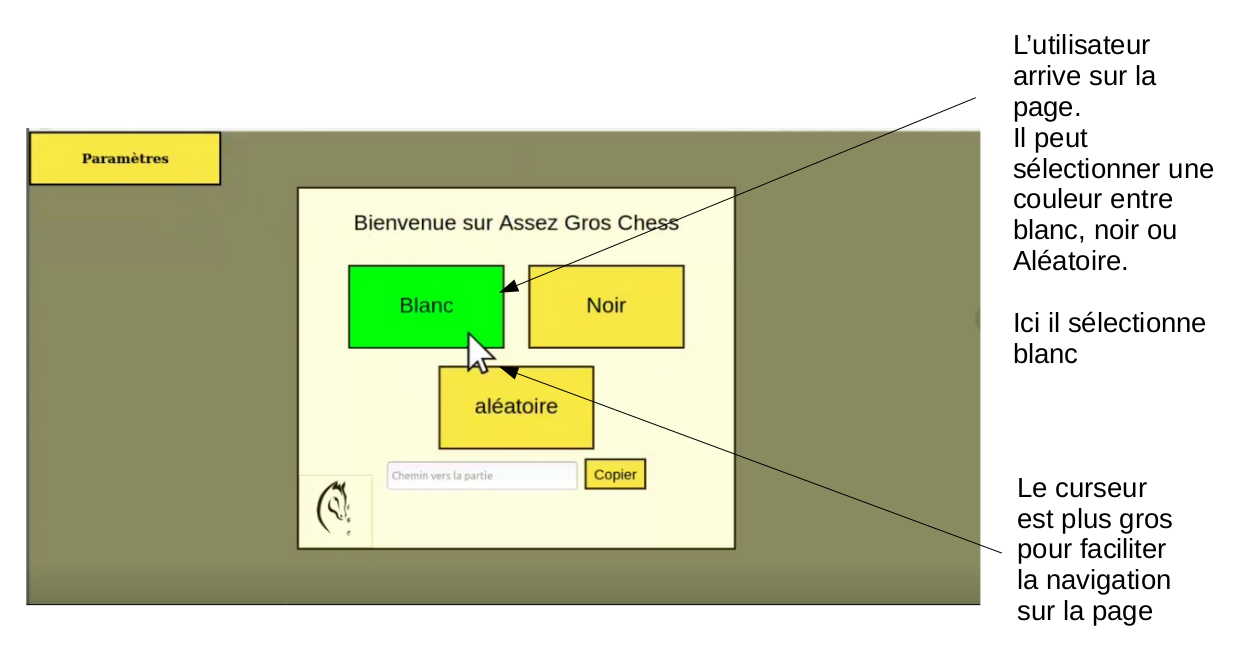
\includegraphics[width=12cm]{UseCase/Accueil1/Accueil1.png}
                   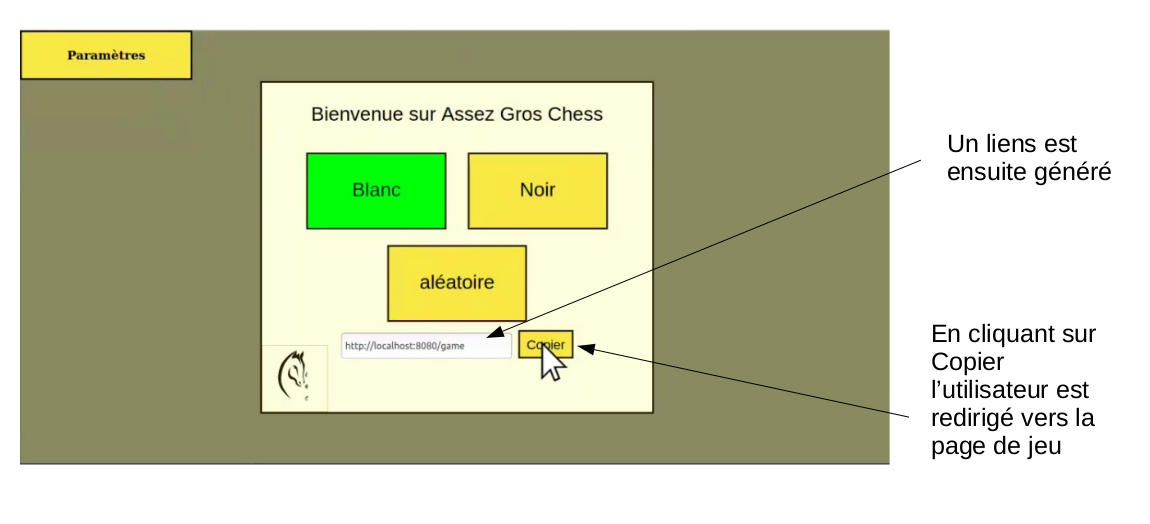
\includegraphics[width=12cm]{UseCase/Accueil1/Accueil2.png}
                    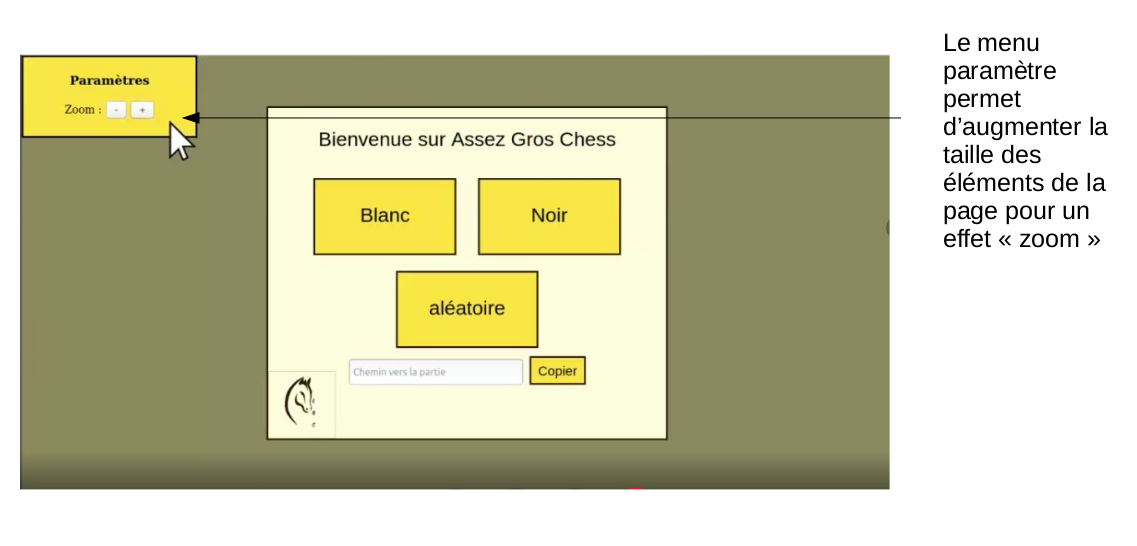
\includegraphics[width=12cm]{UseCase/Accueil1/Accueil3.png}
                    \caption{Page d'accueil}
                \end{figure}

                \begin{figure}
                   \centering 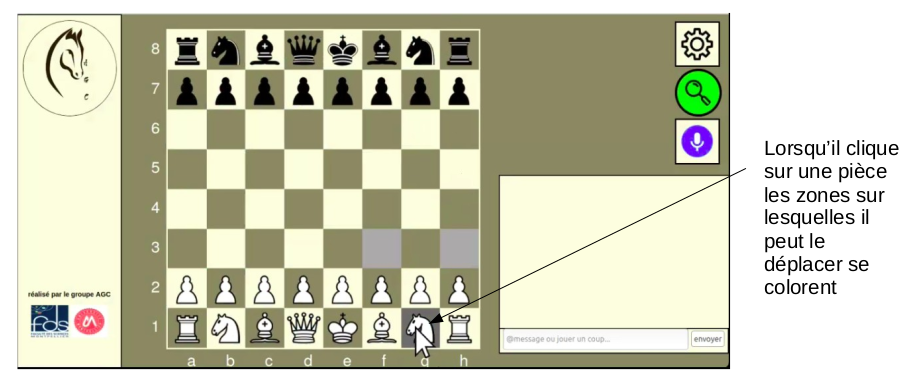
\includegraphics[width=12cm]{UseCase/Jeu1/Game2.png}
                   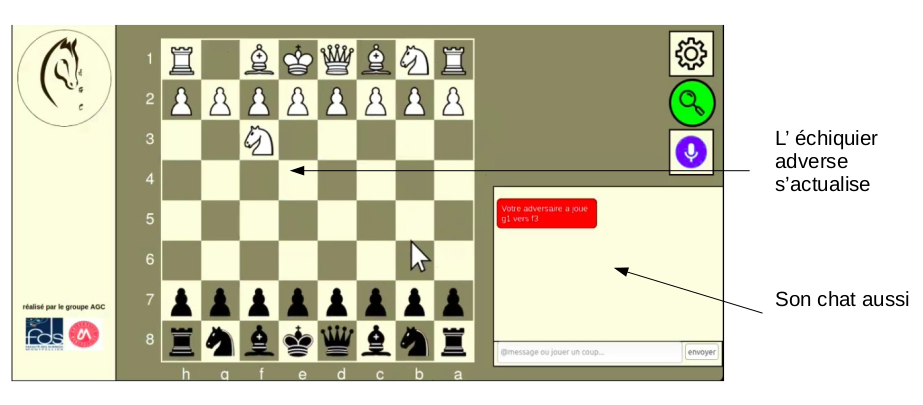
\includegraphics[width=12cm]{UseCase/Jeu1/Game3.png}
                    \caption{Déplacement des pièces}
                \end{figure}
                \begin{figure}
                   \centering 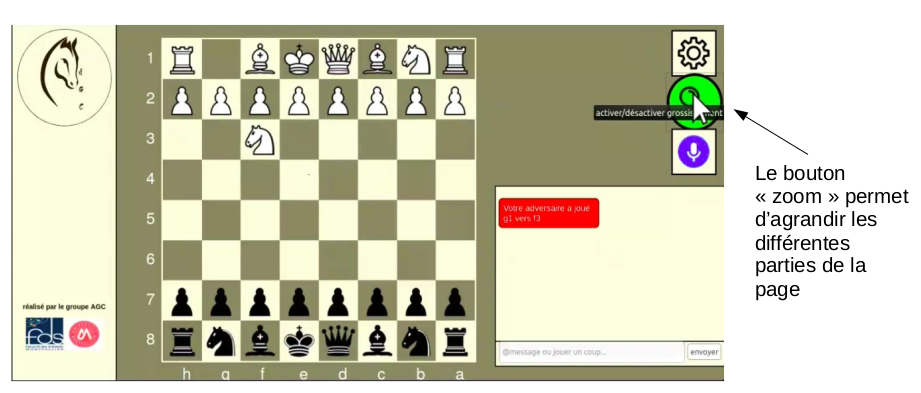
\includegraphics[width=12cm]{UseCase/Jeu1/Game4.png}
                   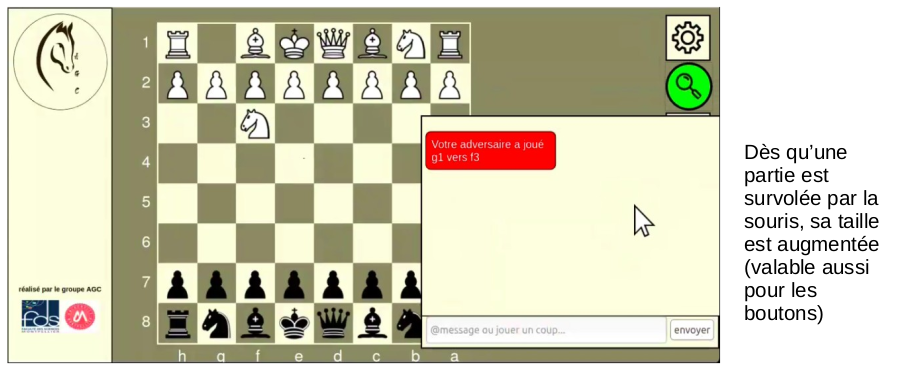
\includegraphics[width=12cm]{UseCase/Jeu1/Game5.png}
                    \caption{Zoom}
                \end{figure} 
                 \begin{figure}
                   \centering 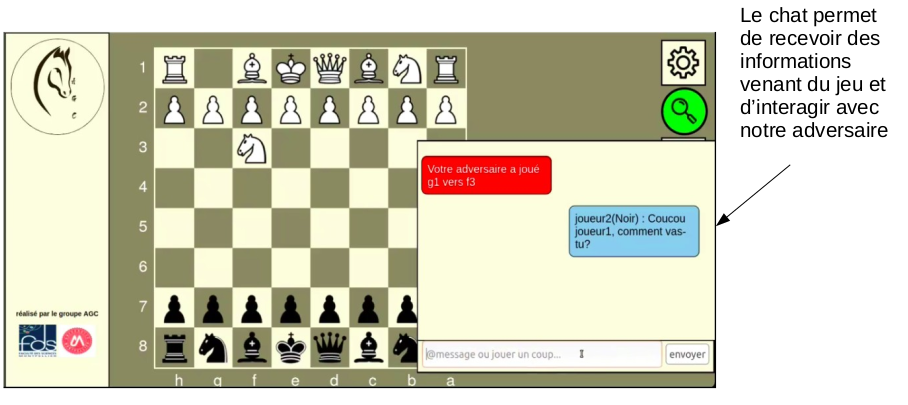
\includegraphics[width=12cm]{UseCase/Jeu1/Game6.png}
                   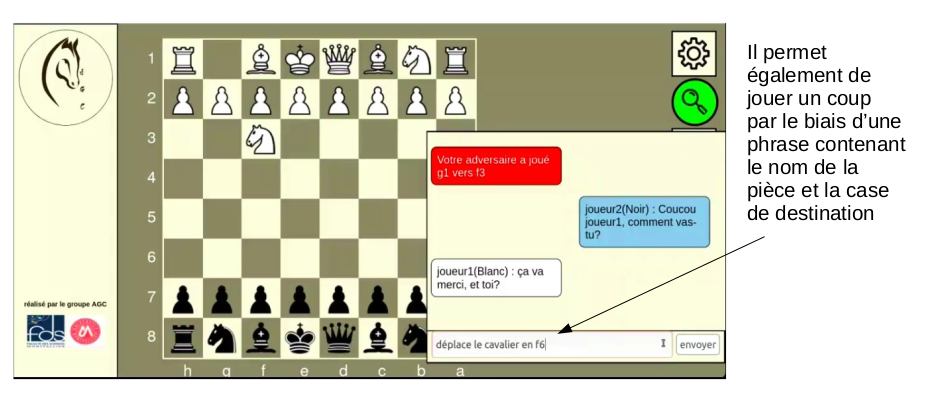
\includegraphics[width=12cm]{UseCase/Jeu1/Game7.png}
                   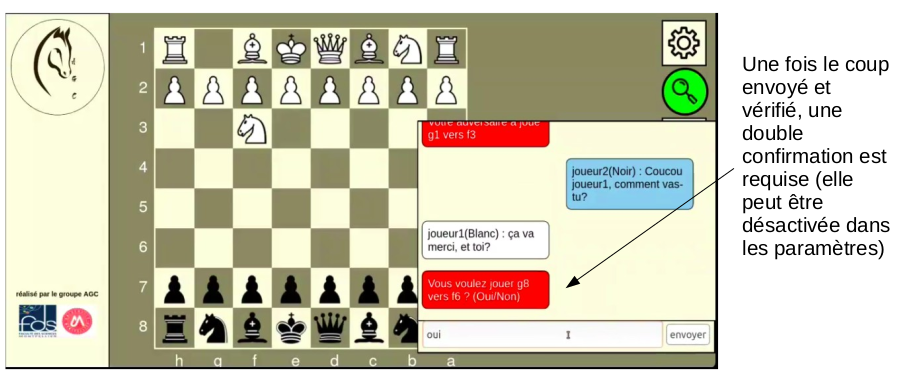
\includegraphics[width=12cm]{UseCase/Jeu1/Game8.png}
                    \caption{Chat}
                \end{figure}
                \begin{figure}
                   \centering 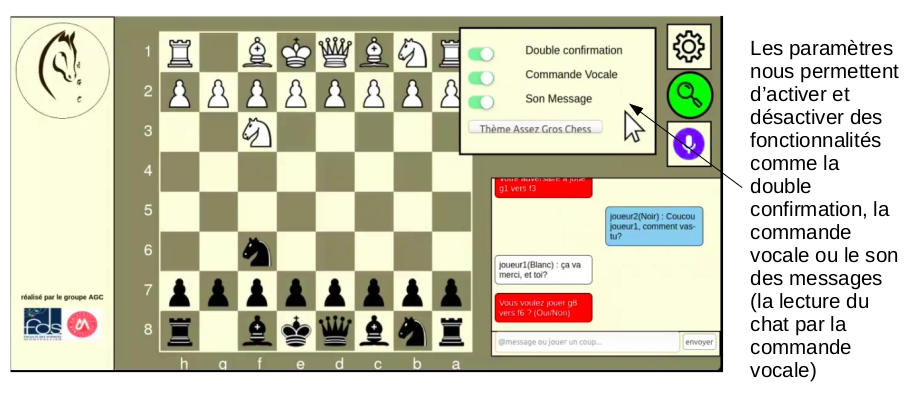
\includegraphics[width=12cm]{UseCase/Jeu1/Game10.png}
                   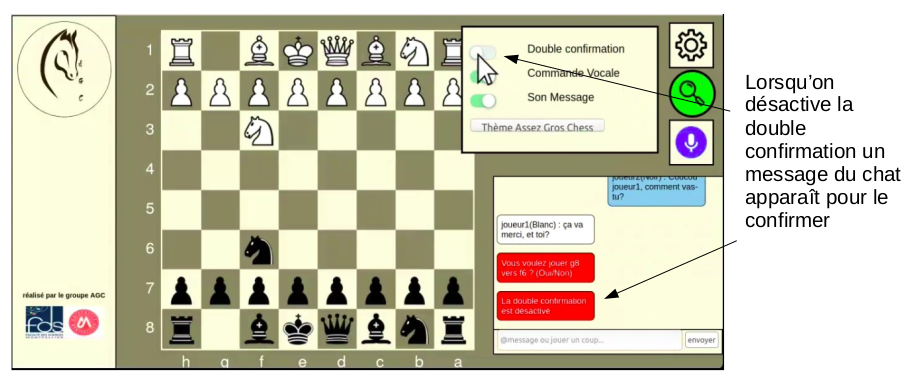
\includegraphics[width=12cm]{UseCase/Jeu1/Game11.png}
                   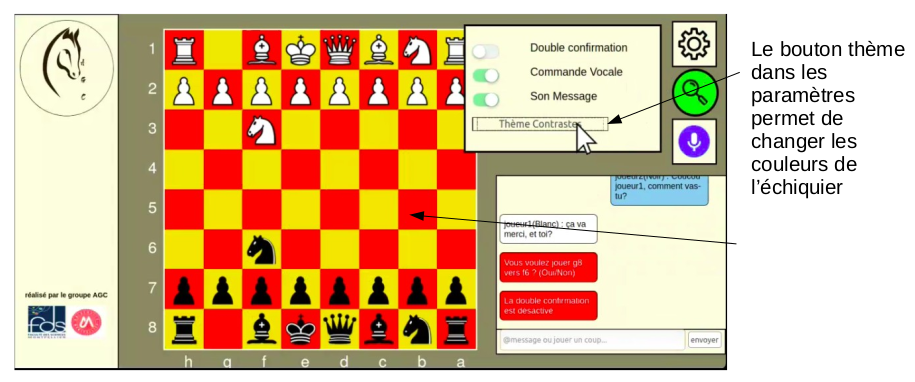
\includegraphics[width=12cm]{UseCase/Jeu1/Game12.png}
                   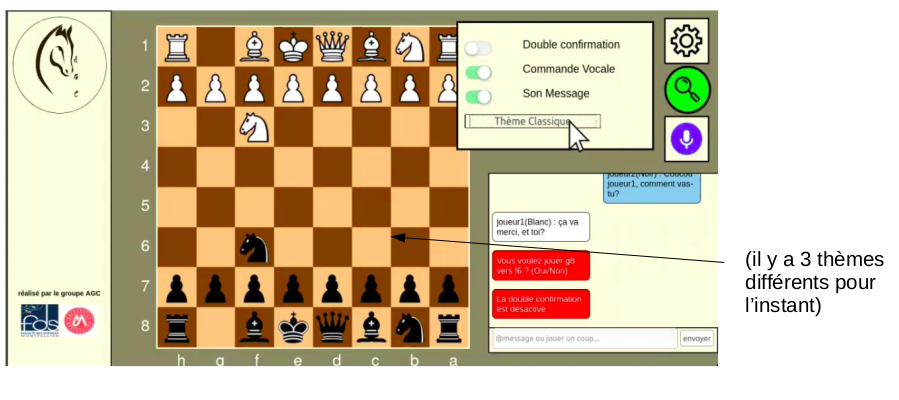
\includegraphics[width=12cm]{UseCase/Jeu1/Game13.png}
                    \caption{Paramètres}
                \end{figure}

    
\end{center}{}

\newpage
\section{Choix des modèles d'architecture} 
Après la conception de notre interface graphique, nous nous sommes penchés sur l'architecture de notre projet.
\subsection{Communication réseau}
Nous avons choisi une architecture client serveur, elle désigne un mode de communication entre plusieurs ordinateurs d’un réseau qui distingue un ou plusieurs postes clients du serveur : chaque logiciel client peut envoyer des requêtes à un serveur. Un serveur peut être spécialisé en serveur d’applications, de fichiers, de terminaux, ou encore de messagerie électronique. Nous avons choisi une telle architecture, car elle permet :
\begin{itemize}
    \item  La centralisation des données sur un seul serveur, ce qui simplifie les contrôles de sécurité, l’administration, la mise à jour des données et des logiciels.
    \item La concentration de la complexité et la puissance de calcul sur le serveur.  
 \end{itemize}{}
\newline
\subsection{Côté serveur}
Afin d'organiser le côté serveur de notre projet, nous avons choisi un modèle d'architecture Modèle/Vue/Contrôleur (MVC). Elle consiste à distinguer trois entités distinctes qui sont, le modèle, la vue et le contrôleur ayant chacun un rôle précis dans l'interface :
\begin{itemize}
    \item modèle : données (accès et mise à jour).
    \item vue : interface utilisateur (entrées et sorties).
    \item contrôleur : gestion des événements et synchronisation.
\end{itemize}{}


Notre choix s'est porté sur cette dernière car elle apporte de réels avantages : 
\begin{itemize}
    \item Meilleure organisation du code.
    \item Diminution de la complexité lors de la conception.
    \item Conception claire et efficace grâce à la séparation des données de la vue et du contrôleur.
    \item Une plus grande souplesse pour organiser le développement du site (répartition des taches plus facile). 
\end{itemize}{}
\subsection{Côté client}
Afin d'organiser le côté client, nous nous sommes inspirés des diagrammes d'interactions utilisés pour rendre compte de l'organisation spatiale des participants à l'interaction. Cette modélisation nous permet de montrer les événements reçu et émis par le client ainsi que les interactions avec le serveur et l'utilisateur. Elle permet également de faire apparaître l'architecture interne, les différents blocs du programme.

\section{Modélisation de l'architecture}
\subsection{Côté serveur}
L'image ci dessous explique l'organisation de la partie Serveur de notre architecture.\newline
 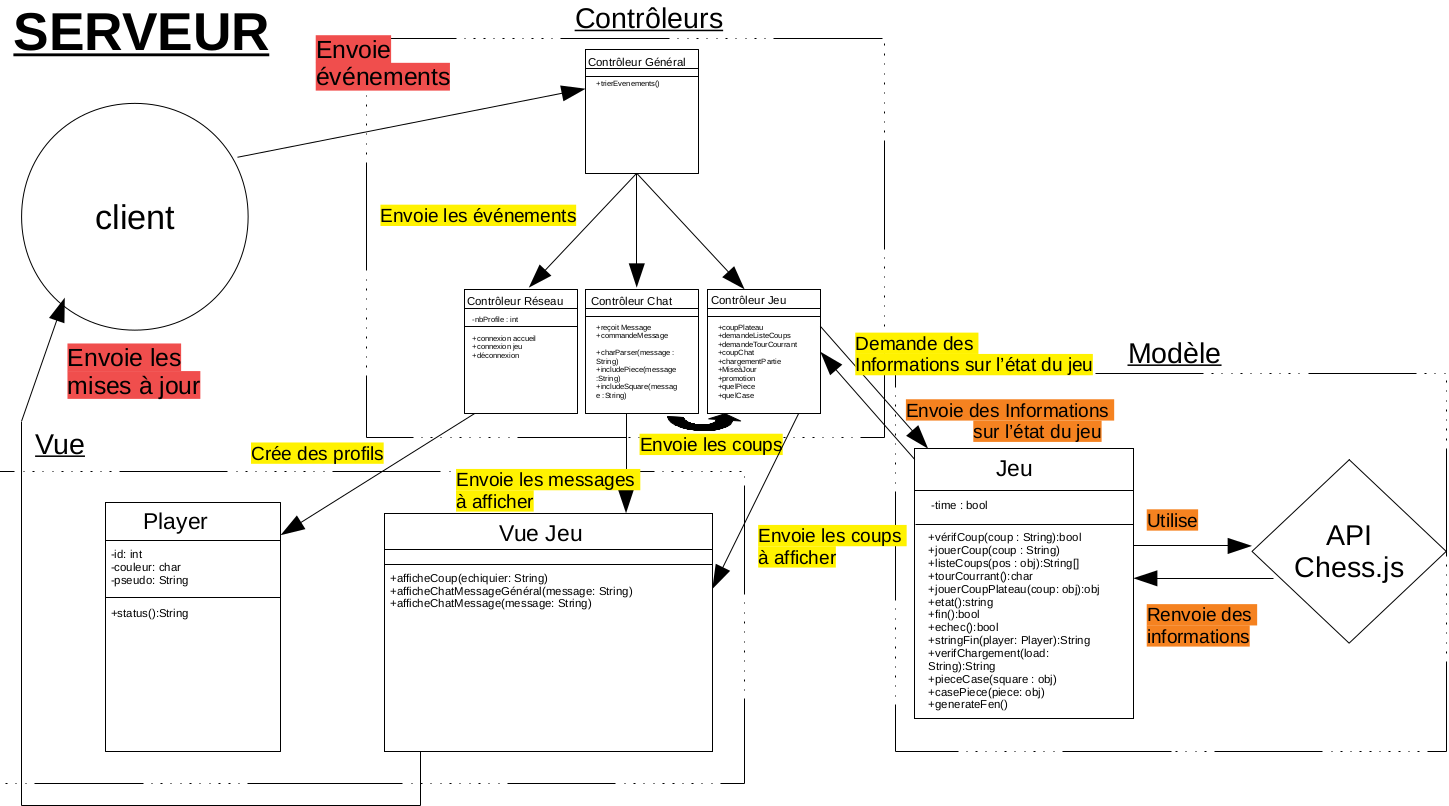
\includegraphics[width=16cm]{Serveur.png}  
Le serveur est composé de trois blocs principaux le Modèle, le Contrôleur et la Vue :
\begin{enumerate}

    \item \textbf {Modèle}: composé d’un bloc « Jeu » en liens avec la bibliothèque « Chess.js » (contenant les fonctionnalités d’un jeu d’échec « standard » (règles, pièces, contraintes de déplacement, condition d’échec, ...)). Celui-ci envoie au Contrôleur jeu les informations sur l'état du jeu demandées.
    \item \textbf {Contrôleur}: composé d'une partie générale, qui trie tous les évènements et les redirigent vers trois sous parties qui traitent chacune des informations spécifiques.
    \begin{enumerate}
        \item \textbf {Contrôleur réseau} : gère les évènements liés aux connexions (nombre de profils, connexion à l’accueil, au jeu) il communique avec l’entité « Joueur » dans la partie Vue.
         \item \textbf {Contrôleur chat} : traite des informations comme la réception des messages, les commandes passant par chat, etc. Il communique principalement avec la partie Vue mais aussi avec le contrôleur jeu (pour vérifier les coups notamment).
          \item \textbf {Contrôleur jeu} : s'occupe des évènements concernant le jeu d’échec. Cela comprend les coups, l’échiquier, le tour de jeu, et bien d’autres (les fonctions modélisés sur le graphique traitent ces informations). Il communique avec le bloc « Jeu » dans la partie Modèle ainsi qu'avec le bloc "Vue Jeu" partie Vue. Par exemple une fois le coup d'un joueur validé par la bibliothèque, le contrôleur jeu le transfert à la Vue, ce qui permet d’actualiser l’échiquier.
     \end{enumerate}{}
    \item \textbf {Vue}: contient deux blocs distincts qui reçoivent des informations venant respectivement des Contrôleurs chat, jeu et réseau.
    \begin{enumerate}
        \item \textbf {Vue Jeu} : permet ainsi d’afficher les messages venant d’un autre utilisateur ou directement du contrôleur Jeu dans le chat, il affiche également les coups sur l’échiquier. Ces mises à jour sont transférés au client. (cf. Figure 1.4)
        \item \textbf {Joueur} : ce dernier enregistrera les informations choisies par le joueur avant que la partie ne commence (son pseudo, la couleur qu’il a choisie de jouer  cf. Figure 2.1).
    \end{enumerate}{}
\end{enumerate}

\subsection{Côté client}

L'image ci dessous explique l'organisation de la partie Client de notre architecture.\newline
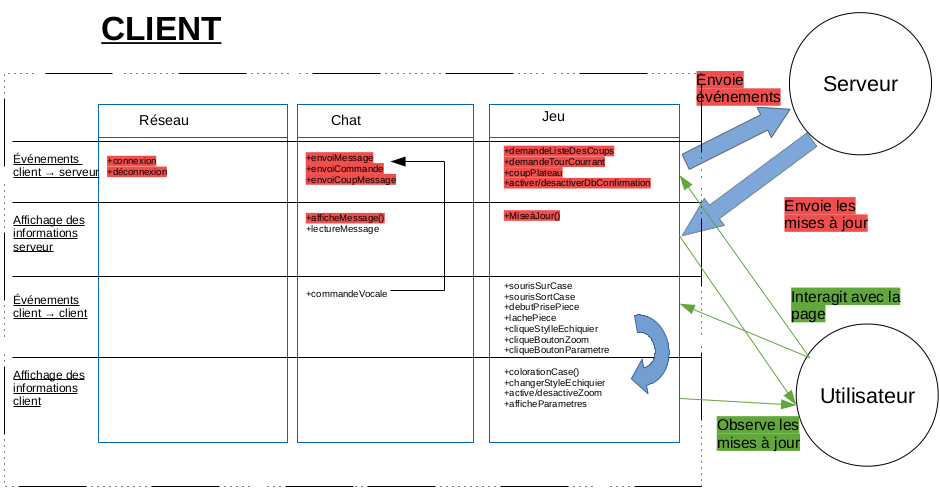
\includegraphics[width=16cm]{Client.png}
On distingue la partie Client contenant 3 blocs (Réseau, Chat et Jeu), l’Utilisateur représenté en bas à droite, et le Serveur au-dessus.
\newline
L’Utilisateur va provoquer différents évènements en interagissant avec la page, et en jouant. Ces évènements sont représentés dans les blocs auxquels ils sont rattachés. On distinguera les évènements envoyés au serveur pour qu’ils soient traités (client→serveur, en rouge sur le schéma), des évènements directement gérés par la page. (client→client, en blanc)
\newline
Pour mieux commprendre comment fonctionne cette partie nous avons choisit deux exemples:
\begin{enumerate}
    \item \textbf {Utlisation de la commande vocale} : quand un joueur utilise cette dernière pour jouer un coup, par exemple. L’évènement « commande Vocale » est géré par la page, qui activera la fonction nécessaire directement. Cet évènement provoque ensuite un autre évènement dans le chat, pour envoyer le coup au serveur « envoiCoupMessage ». Le serveur renvoie par la suite, les mises à jour (comme une double vérification si nécessaire, ou simplement l’échiquier actualisé).
    \item \textbf {Changement du thème} : si l’utilisateur choisi de changer le thème de son échiquier (cf. Figure 1.5 Paramètres), l’évènement « changerStyleEchiquier » sera géré directement par la page, et les mises à jours seront observées par le client.
\end{enumerate}{}




\chapter{Implementation}

\section{Choix des langages}

Comme nous avons choisi de développer Assez Gros Chess sur un modèle client-serveur, le choix des langages de programmation est lui aussi impacté.

Coté client HTML,CSS et JavaScript s'imposent. De plus, tous les membres du groupe possèdent déjà des bases dans ces deux premiers et le JavaScript est un langage simple à appréhender.
Coté Serveur, nous avons choisi de nous orienter vers nodeJs qui va nous permettre de garder une continuité dans le langage entre la partie client et la partie serveur puisque cette plateforme nous offre un environnement permettant d'exécuter du code JavaScript coté serveur. De plus, nodeJS va nous permettre de manière très simple la mise en place de notre serveur et permet également d'accéder à une grande quantité de modules (équivalent des librairies) facilement via npm (Node Package Manager, ou en français : Gestionnaire des paquets de Node). 

Nous utilisons ici les dernières versions de chaque technologie à savoir:
\begin{itemize}
    \item HTML 5
    \item CSS 3
    \item JavaScript ES6
    \item NodeJS v12
\end{itemize}

Nous utiliserons également pour ce projet un certain nombre de bibliothèques dont le choix et l'utilisation seront détaillés par la suite.

\begin{itemize}
    \item Chess.js
    \item WebSpeechAPI
    \item Socket.io
    \item Express Framework
    \item chessboard.js
\end{itemize}

\newpage
\section{Communication réseau}

Pour la communication client-serveur plusieurs possibilités s'offrent à nous.
Nous avons choisi d'utiliser un système de sockets avec le module socket.io disponible dans npm.
Ce type de communication correspond bien à nos besoins, car elle est en temps réel et bidirectionnelle, ainsi le serveur peut envoyer des informations au client et vis versa. De plus, elle se base sur des évènements et s'accorde donc parfaitement avec NodeJS qui est non-bloquant et fonctionne également par évènements.

Côté serveur on démarre le serveur WebSocket qui sera associé au serveur HTTP, celui-ci "écoute" également sur le même port.

\begin{verbatim}
    const io = require('socket.io').listen(server);
    io.sockets.on('connection', function (socket, player) {
        
    });
\end{verbatim}

Lorsqu'un client se connecte sur la page, un script js démarre la connexion WebSocket. 

\begin{verbatim}
    var socket = io.connect('http://localhost:8080');
\end{verbatim}
(note : dans cet exemple les connexions sont faites en local)

À partir de ce moment les 2 programmes peuvent "dialoguer" via des évènements.
(voir Annexe 3.2 pour le schéma)

\newpage
\section{Implémentation du programme Côté serveur : Moteur}

\subsection{Mise en place du serveur}

Nous avons donc choisi de mettre en place un serveur avec l'aide de NodeJS plutôt que d'utiliser des serveurs existants comme Apache.

Nous avons utilisé le framework express pour la mise en place de celui-ci. Il est disponible sur npm et va nous permettre de gérer simplement les requêtes, les routes, le rendu des vues HTML, les cookies, l'authentification, etc. Comme le ferait un serveur Apache.

Ainsi, nous pouvons créer un serveur en seulement quelques lignes, il nous suffit de charger le module, définir les principales routes et le port sur lequel il doit écouter.

\begin{verbatim}
const express = require('express');
const app = express();
const server = require('http').createServer(app);

app.use(express.static(__dirname + '/HTML/'));

app.get('/', function (req, res) {
    res.sendFile(path.join(__dirname + '/HTML/index.html'));
});

app.get('/game', function (req, res) {
    res.sendFile(path.join(__dirname + '/HTML/game.html'));
});

server.listen(80);
\end{verbatim}

\subsection{Gestion des évènements}

Notre programme va être amené à gérer différents types d'évènements concernant le jeu, le chat, les connexions...
Nous avons donc pris l'initiative de créer une classe de contrôle général des évènements dont le rôle sera de répartir les différents évènements dans les différents blocs auxquels ceux-ci sont liés.

Ainsi, au lancement du serveur, celui-ci crée une instance de cette classe puis celle-ci reçoit les évènements et les renvoie aux classes qui contrôlent le jeu, le chat ou le réseau.\newline
(partie de code en annexe 3.3.2)

\newpage
\subsection{Gestion des joueurs}

La gestion des joueurs se fait assez simplement car socket.io va nous permettre de mémoriser les différents clients. En effet, lorsqu'un nouveau client se connecte au serveur, celui-ci va instancier un nouvel objet de type socket. Il existe donc un objet socket pour chaque client qui est stocké côté serveur. On va donc pouvoir retenir des informations concernant les différents clients sous forme de variables de sessions.

Nous avons créé une classe joueur qui va nous permettre de sauvegarder différentes informations sur les joueurs (id, couleur, pseudo) et tout cela côté serveur uniquement.

Ainsi lors de la première connexion du socket au serveur WebSocket, on crée une nouvelle instance de la classe joueur.\newline
(partie de code en annexe 3.3.3)

\subsection{La partie d'échec}

Étant donné le temps dont nous disposions, nous avons décidé de ne pas recréer un jeu d'échec entier afin de nous concentrer d'avantage sur l'interface et la communication.

Nous avons donc utilisé l'API chess.js (disponible sur npm) qui est un moteur de jeu d'échec. De plus, cette API est utilisée par de nombreux site d'échec en ligne comme lichess.org (qui est une référence en tant que site d'échec). Elle fournit une documentation complète des fonctionnalités et peut être utilisée avec n'importe quel type d'interface. 

L'interaction avec Chess.js se fait de la façon suivante :
\begin{itemize}
    \item Dans notre cas, elle sera donc utilisée exclusivement côté serveur puisque la partie est commune aux deux joueurs. 
    \item La classe Game est la seule classe du programme à pouvoir dialoguer avec l'API.
    \item Le contrôleur de jeu fait appel à la classe Game lors de différents évènements.
\end{itemize}

Exemple de situation :

\begin{center}
    \centering
    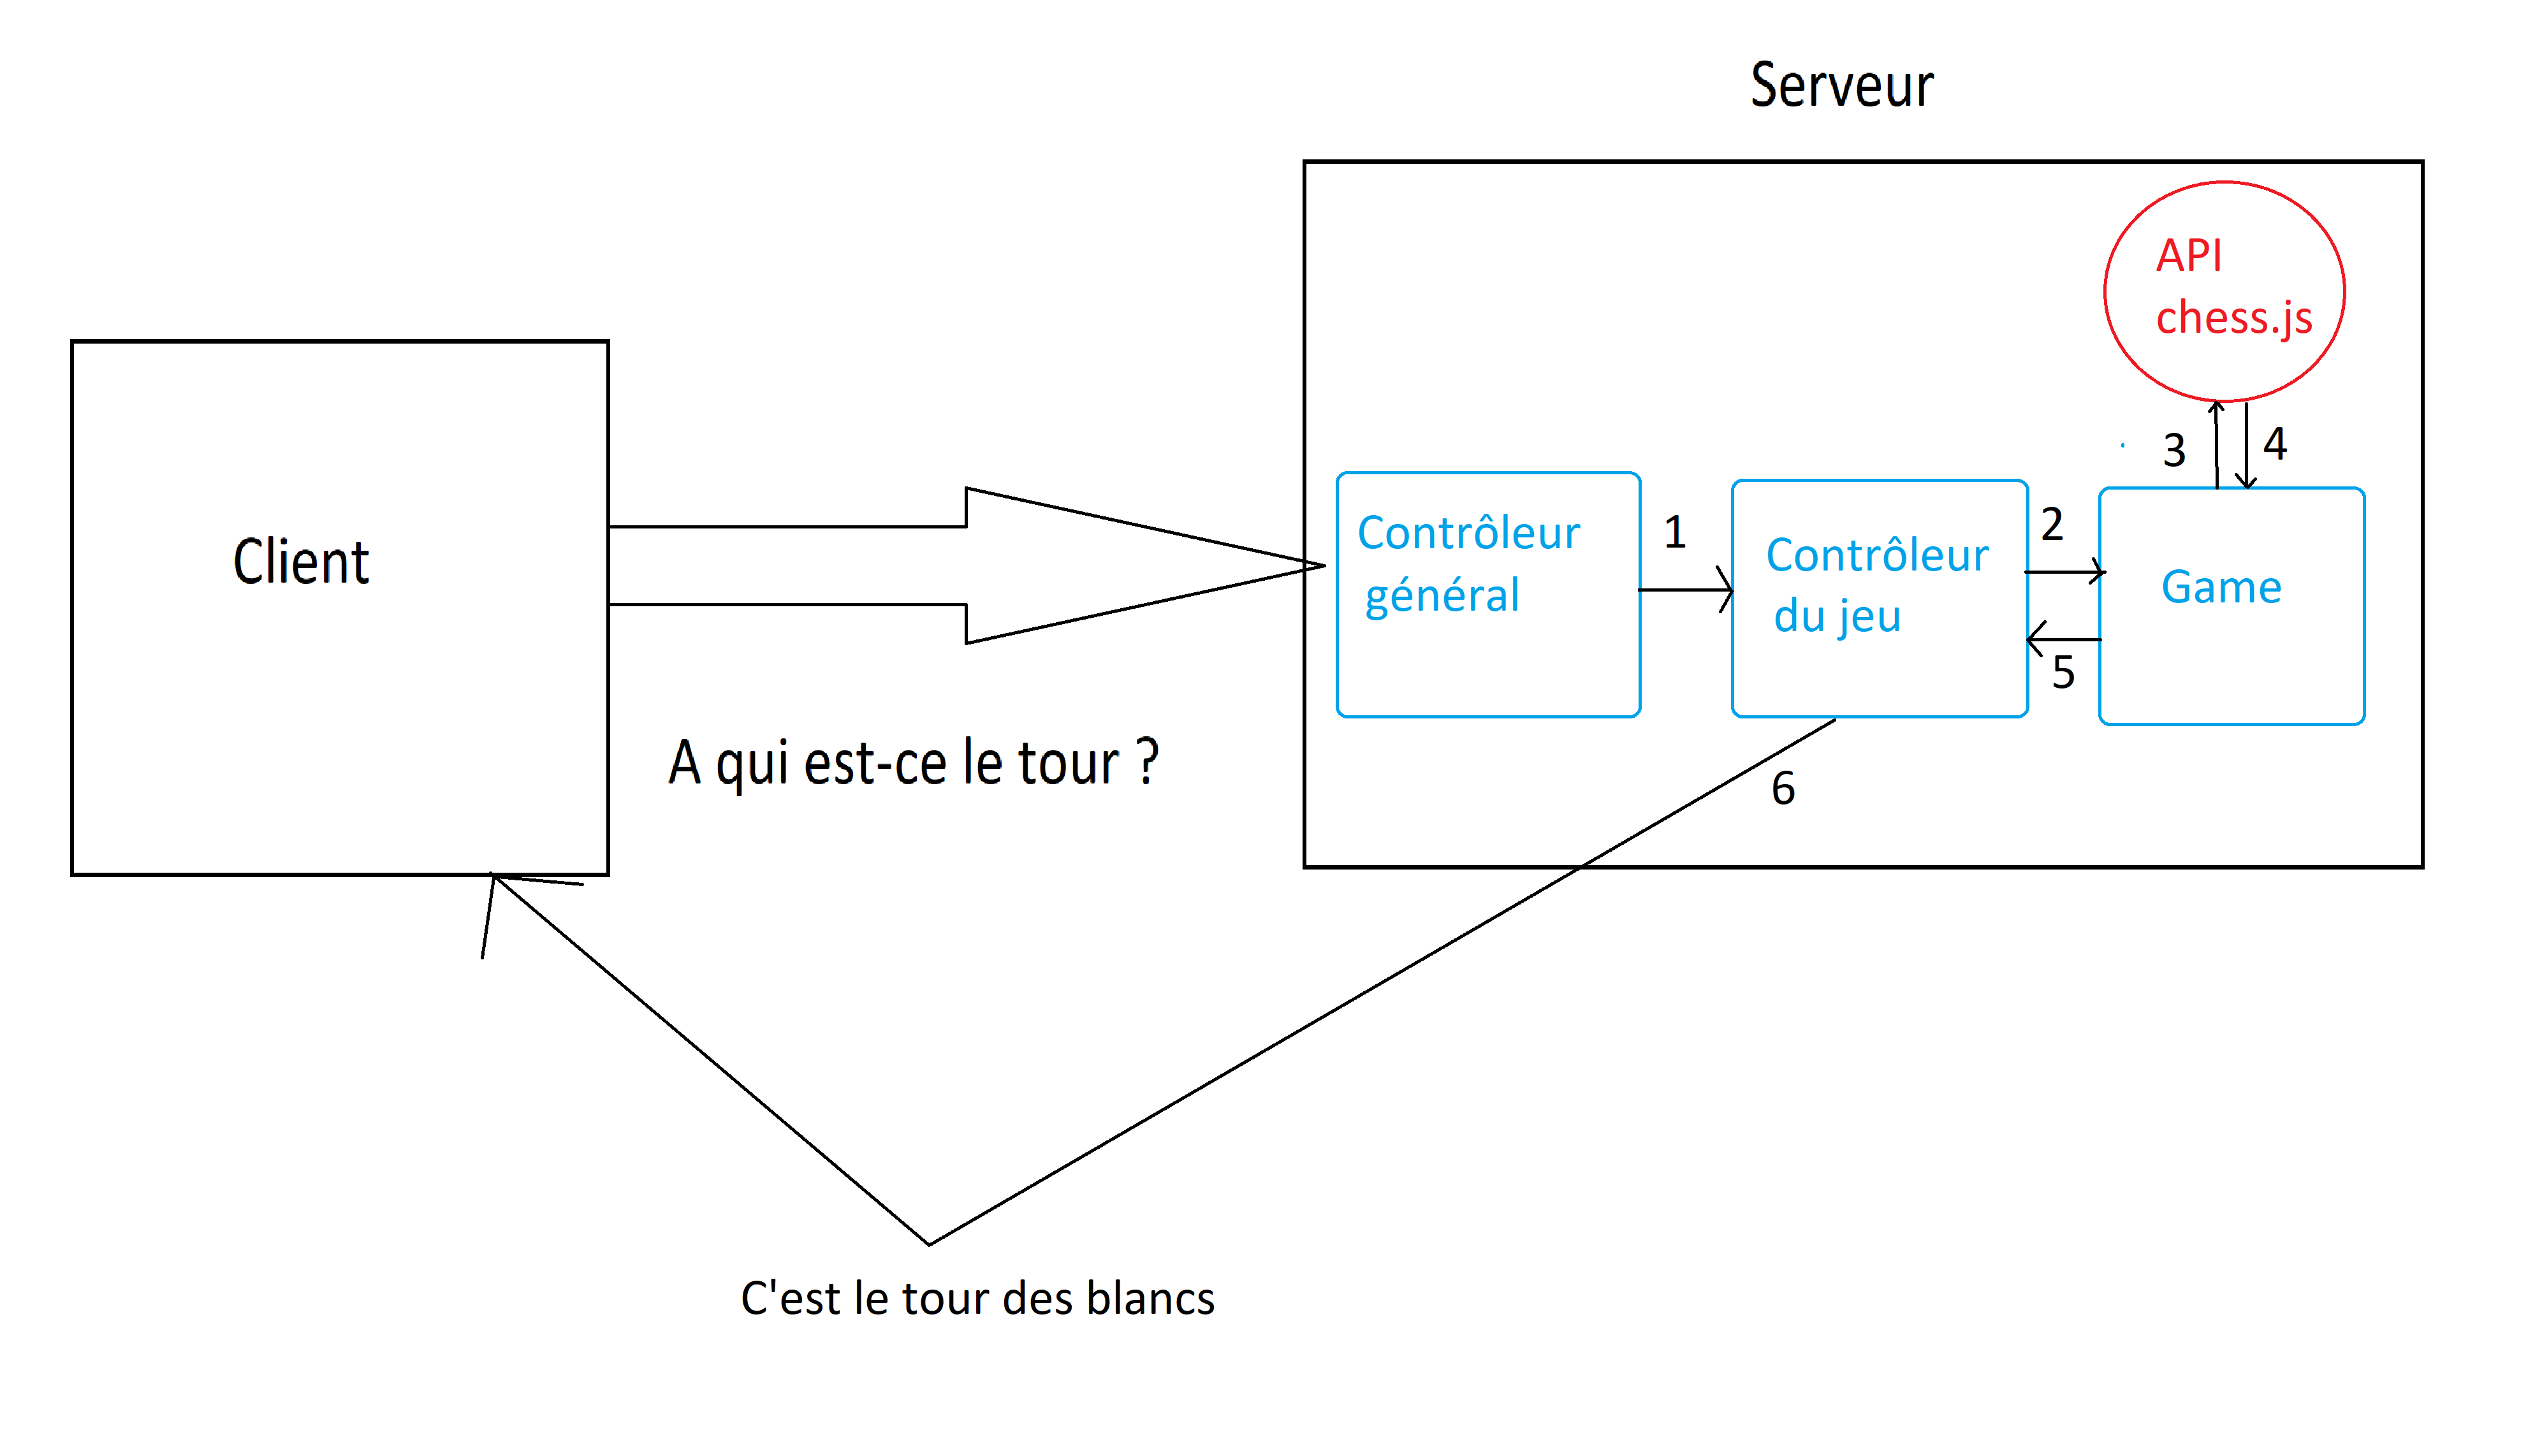
\includegraphics[width=14cm]{src/image4.png}
\end{center}

Explication : \newline
Le logiciel client veut connaître le tour courant.
Il envoie une requête au serveur.
Le serveur reçoit un évènement, il est trié par le contrôleur générale pour arriver dans le contrôleur du jeu.
Le contrôleur du jeu demande à la classe Game quel est le tour courant.
Celui-ci répond en utilisant l'API.
Le contrôleur du jeu renvoie la réponse au logiciel client.



\subsection{Le chat}

La réalisation du chat a été l'une des parties les plus importantes du projet.
Pour rappel, le chat doit permettre de dialoguer avec son adversaire, de jouer des coups, de demander la position des pièces, mais également une implémentation simple de la commande vocale par la suite.

Pour cela il existe donc une classe dédiée au contrôle du chat. Cette classe dispose de plusieurs fonctions afin de "parser", d'analyser les messages du chat. Elle reçoit un seul type d'évènements qui sont les messages envoyés par les joueurs et elle peut également communiquer avec le contrôleur de jeu.

Fonctionnement :

Lorsqu'un message est reçu, on regarde dans un premier temps :
\begin{itemize}
    \item Si le message commence par @, c'est alors un message destiné à l'adversaire. On fait donc suivre le message à la classe view qui s'occupe de renvoyer les informations à afficher aux clients.
    \item Si le message commence par /, c'est alors une commande pour le serveur. Ils existent seulement quelques-unes et permettent par exemple de charger un état.
\end{itemize}

Si aucun des deux cas précédent n'est vérifié alors il va falloir analyser le contenu du message.
\newline\newline
\textbf{Choix d'implémentation}

On souhaite analyser le chat afin de réaliser des actions différentes en fonction du contenu des messages, ainsi plusieurs options s'offrent à nous.
\begin{itemize}
    \item Une première solution consiste à recenser dans un dictionnaire la liste des mots qui peuvent potentiellement être utilisés. Par exemple : des verbes d'action (déplace, bouge, met...), des pronoms interrogatifs (ou), des prépositions (avec, sur, en...). 
    \begin{itemize}
        \item  L'avantage de cette méthode et que seuls quelques schémas de phrases sont acceptés, le résultat sera donc toujours celui souhaité.
        \item  Ses inconvénients sont qu'elle est plus longue à implémenter et que le programme ne saura pas s'adapter face à des cas de figure imprévus.
    \end{itemize}
    \item La deuxième solution consiste à uniquement relever quelques mots les plus importants ainsi que leur nombre d'apparitions, puis d'essayer d'en déduire la situation la plus probable. Par exemple, si la phrase contient uniquement un nom de case, il ne peut pas s'agir d'un mouvement puisqu'on ne sait pas quelle pièce, il faudrait déplacer. 
    \begin{itemize}
        \item L'avantage de cette méthode est qu'elle s'adapte à tout type de phrases et est plus simple à implémenter.
        \item L'inconvénient est que le programme peut effectuer la mauvaise action si on n'interprète pas bien le contenu de la phrase.
    \end{itemize}
\end{itemize}
Nous avons finalement choisi la seconde méthode par soucis de simplicité et afin que le programme puisse s'adapter à des phrases inconnues.

\textbf{La fonction de parsage}
\newline
La fonction de "parsage" va, grâce à  des expressions régulières permettre de savoir si le message contient des noms de pièces ou encore des emplacements.
Si le message n'en contient aucun, on retourne un message d'erreur à l'utilisateur.\newline
Sinon il existe 4 cas possibles :
\begin{itemize}
    \item Le message comporte uniquement un nom de case. L'utilisateur veut donc savoir quelle pièce se trouve sur cette case. Il s'agit d'un message du type : "Quelle pièce se trouve en A5?".
    \item Le message comporte uniquement un nom de pièce. L'utilisateur veut donc savoir où se trouve la ou les pièces en question. Il s'agit d'un message du type : "Où se trouvent les fous ?".
    \item Le message comporte un nom de pièce et une case.
    Il s'agit alors d'un déplacement simple, par exemple : "Déplace le fou en a5." ou encore "Avance la tour jusqu'en h8".
    \item Le message comporte deux noms de pièce et une case. Il s'agit alors d'une prise de pièce. C'est un message du type : "Prends le fou avec la reine en e4" ou "Le pion prend la tour en d7". (Petite spécificité pour ce cas, il faut gérer le mode passif également).
\end{itemize}
On envoie ensuite en fonction du cas les informations au contrôleur de jeu qui s'occupera de faire les actions adéquates.
(code en annexe 3.3.5)

\newpage
\section{Implémentation du programme côté client : Interface}

L'avantage d'avoir organisé le code sur ce modèle est que l'interface est gérée uniquement côté client ce qui va permettre d'offrir des interfaces différentes en fonction des clients.
Nous avons réalisé différentes feuilles de style CSS pour les différentes parties de l'interface, le code JavaScript vient s'ajouter en complément.

\subsection{L'échiquier}

Assez Gros Chess est avant tout un jeu d'échec, donc l'élément principal de l'interface se doit d'être l'échiquier.
Celui-ci se doit d'être visible, modulable et doit pouvoir interagir avec du code JavaScript pour se mettre à jour.

Afin de nous simplifier la tâche, nous avons utilisé une petit API appelée chessboard.js, celle-ci permet simplement d'afficher les pièces sur l'échiquier et de pouvoir les glisser-déposer.
Nous avons ensuite fait en sorte :
\begin{itemize}
    \item Qu'on ne puisse pas interagir avec l'échiquier lorsque ce n'est pas notre tour.
    \item Qu'on puisse sélectionner une pièce et que cela nous surligne les coups possibles.
    \item Que l'on puisse déplacer une pièce avec de simples cliques sur l'écran.
    \item Qu'on puisse changer la couleur de l'échiquier.
\end{itemize}
.
\newline
\textbf{Problème rencontré lors de l'implementation}
\newline
Ce paragraphe traite exclusivement d'un problème que nous avons rencontré lors de l'implémentation de l'échiquier.

En effet, la conception originelle ne comportait dans la section jeu que la gestion des évènements joués coups chat/plateau. Ainsi, seul le modèle avait besoin de la liste des coups disponible ainsi que du tour courant.

Or la partie client avait également besoin de cette information afin de savoir quelles sont les cases à surligner et si le joueur a le droit de bouger les pièces en utilisant la souris.
Nous avons donc dû ajouter au contrôleur de jeu la gestion de nouveaux évènements qui sont simplement des demandes d'information de la page concernant les coups possibles ou le tour de jeu courant.


\subsection{Le chat}

Il est constitué d'une zone de texte et d'un champ de saisie. Il permet d'envoyer des messages, ceux-ci se retrouvent dans la zone juste au-dessus et son séparés/colorés selon l'envoyeur. Il est possible de scroller pour revenir vers d'anciens messages. Lorsqu'un message est reçu, nous avons fait en sorte que les derniers messages reçus s'affichent.
(partie de code en annexe 3.4.2)

\newpage
\subsection{Le contrôle Vocale}

Nous avons pensé que l'implémentation d'un contrôle vocale serait un gros plus pour une application destinée à des malvoyants ou même afin de la rendre accessible à des aveugles par la suite.

Le contrôle vocale se fait du côté client uniquement.
Nous avons utilisé l'API WebSpeech qui permet :
\begin{itemize}
    \item une reconnaissance vocale (transforme de la voix en texte)
    \item une synthèse vocale (permet de lire du texte)
\end{itemize} 

La reconnaissance vocale va simplement envoyer au serveur la chaîne de texte obtenue comme un message entré dans le chat.
La synthèse vocale va lire les messages qui s'affichent dans le chat, elle est désactivable via une option.

(partie de code disponible en annexe 3.4.3)

\subsection{Les paramètres et le grossissement}

Les deux boutons restants permettent de gérer ces fonctionnalités.

Les paramètres sont des boutons qui vont modifier les valeurs de certaines variables JavaScript, permettant ainsi d'activer/désactiver des fonctionnalités.

Le grossissement est réalisé entièrement en JavaScript pour chacun des éléments de la page.
(code en annexe 3.4.4)

\section{Quelques Statistiques}

Technologies utilisées
\begin{center}
    \centering
    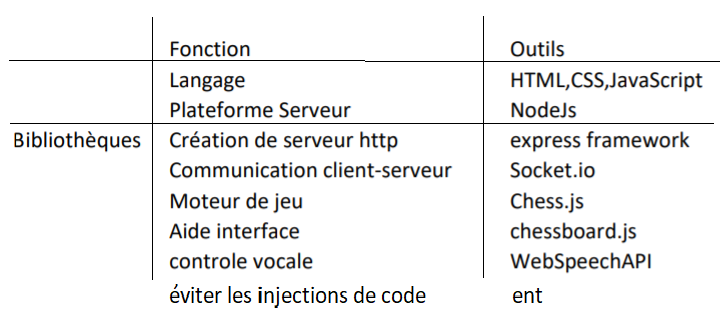
\includegraphics[width=9cm]{src/image5.png}
\end{center}

\begin{itemize}
    \item Nombre de fichiers : 17
    \item Nombre de classes : 7
    \item Nombre de lignes : 1516
\end{itemize}

\chapter{Bilan}
\section{Analyse des résultats obtenus}
\subsection{Couverture des besoins}

Afin de veiller au bon développement de l'application et de bien réussir à couvrir tous les besoins, nous nous étions donné des objectifs à atteindre et nous avons réussi.

\newline
\newline
\textbf{Il est possible de lancer une partie depuis une interface adaptée.}\newlin Le lancement de la partie est simple et intuitif. L'interface est composée de seulement quelques boutons et est modulable.
\newline
\newline
\textbf{Les joueurs sont capables de jouer au jeu d'échec malgré leur trouble visuel.}\newline Le plateau est adapté, il existe différentes couleurs afin de le rendre distinguable. Il est possible de jouer des coups simplement en cliquant, mais aussi via l'utilisation du clavier ou de la voix ce qui rend le jeu accessible au plus grand nombre.
\newline
\newline
\textbf{Les joueurs sont également capable de communiquer entre-eux via le chat}\newline. La taille du chat est variable afin de faciliter la lecture et on peut également écouter les messages grâce à la synthèse vocale.
\newline
\newline
\textbf{L'interface est modulable pour s'adapter au mieux aux joueurs.}\newline Ainsi, les joueurs peuvent à leur convenance, activer ou désactiver certaines fonctionnalités telles que la double confirmation des coups, le grossissement ou encore la commande vocale. Il leur est également possible de zoomer sur les parties de l'interface qu'ils souhaitent visualiser.
\newline
\newline

Ainsi, deux joueurs malvoyants sont capables de jouer en ligne sur notre application dans de bonnes conditions. Il dispose d'une interface adaptée et d'outils pour les aider. 

\subsection{Ce que permet Assez Gros Chess}

\begin{itemize}
    \item Lancer une partie en ligne avec le joueur de notre choix simplement et avec une interface adaptée.
    \item Jouer aux échecs avec des outils d'aide pour les malvoyants, comme des grossissements ou la commande vocale.
    \item Communiquer avec son adversaire et interagir avec le jeu via un chat.
    \item Modifier certaines options via un menu paramètre afin d'adapter l'interface.
    
\end{itemize}

\section{Manques et perspectives d'amélioration}
\subsection{Ce qu'Assez Gros Chess ne permet pas}

\begin{itemize}
    \item La possibilité de jouer pour les joueurs complètement aveugles.
    \item Une gestion des joueurs avec des comptes, ect.
    \item Une plateforme permettant les créations de multiples sessions de jeu (pour le moment, il n'est pas possible de créer qu'une session la fois.)
\end{itemize}
\subsection{Perspectives}

\subsubsection{Rendre le jeu accessible pour les aveugles}

En effet, bien que le jeu implémente une commande vocale ce qui devrait permettre le rendre accessible aux aveugles, il faut actuellement cliquer sur un bouton pour activer cette dernière.

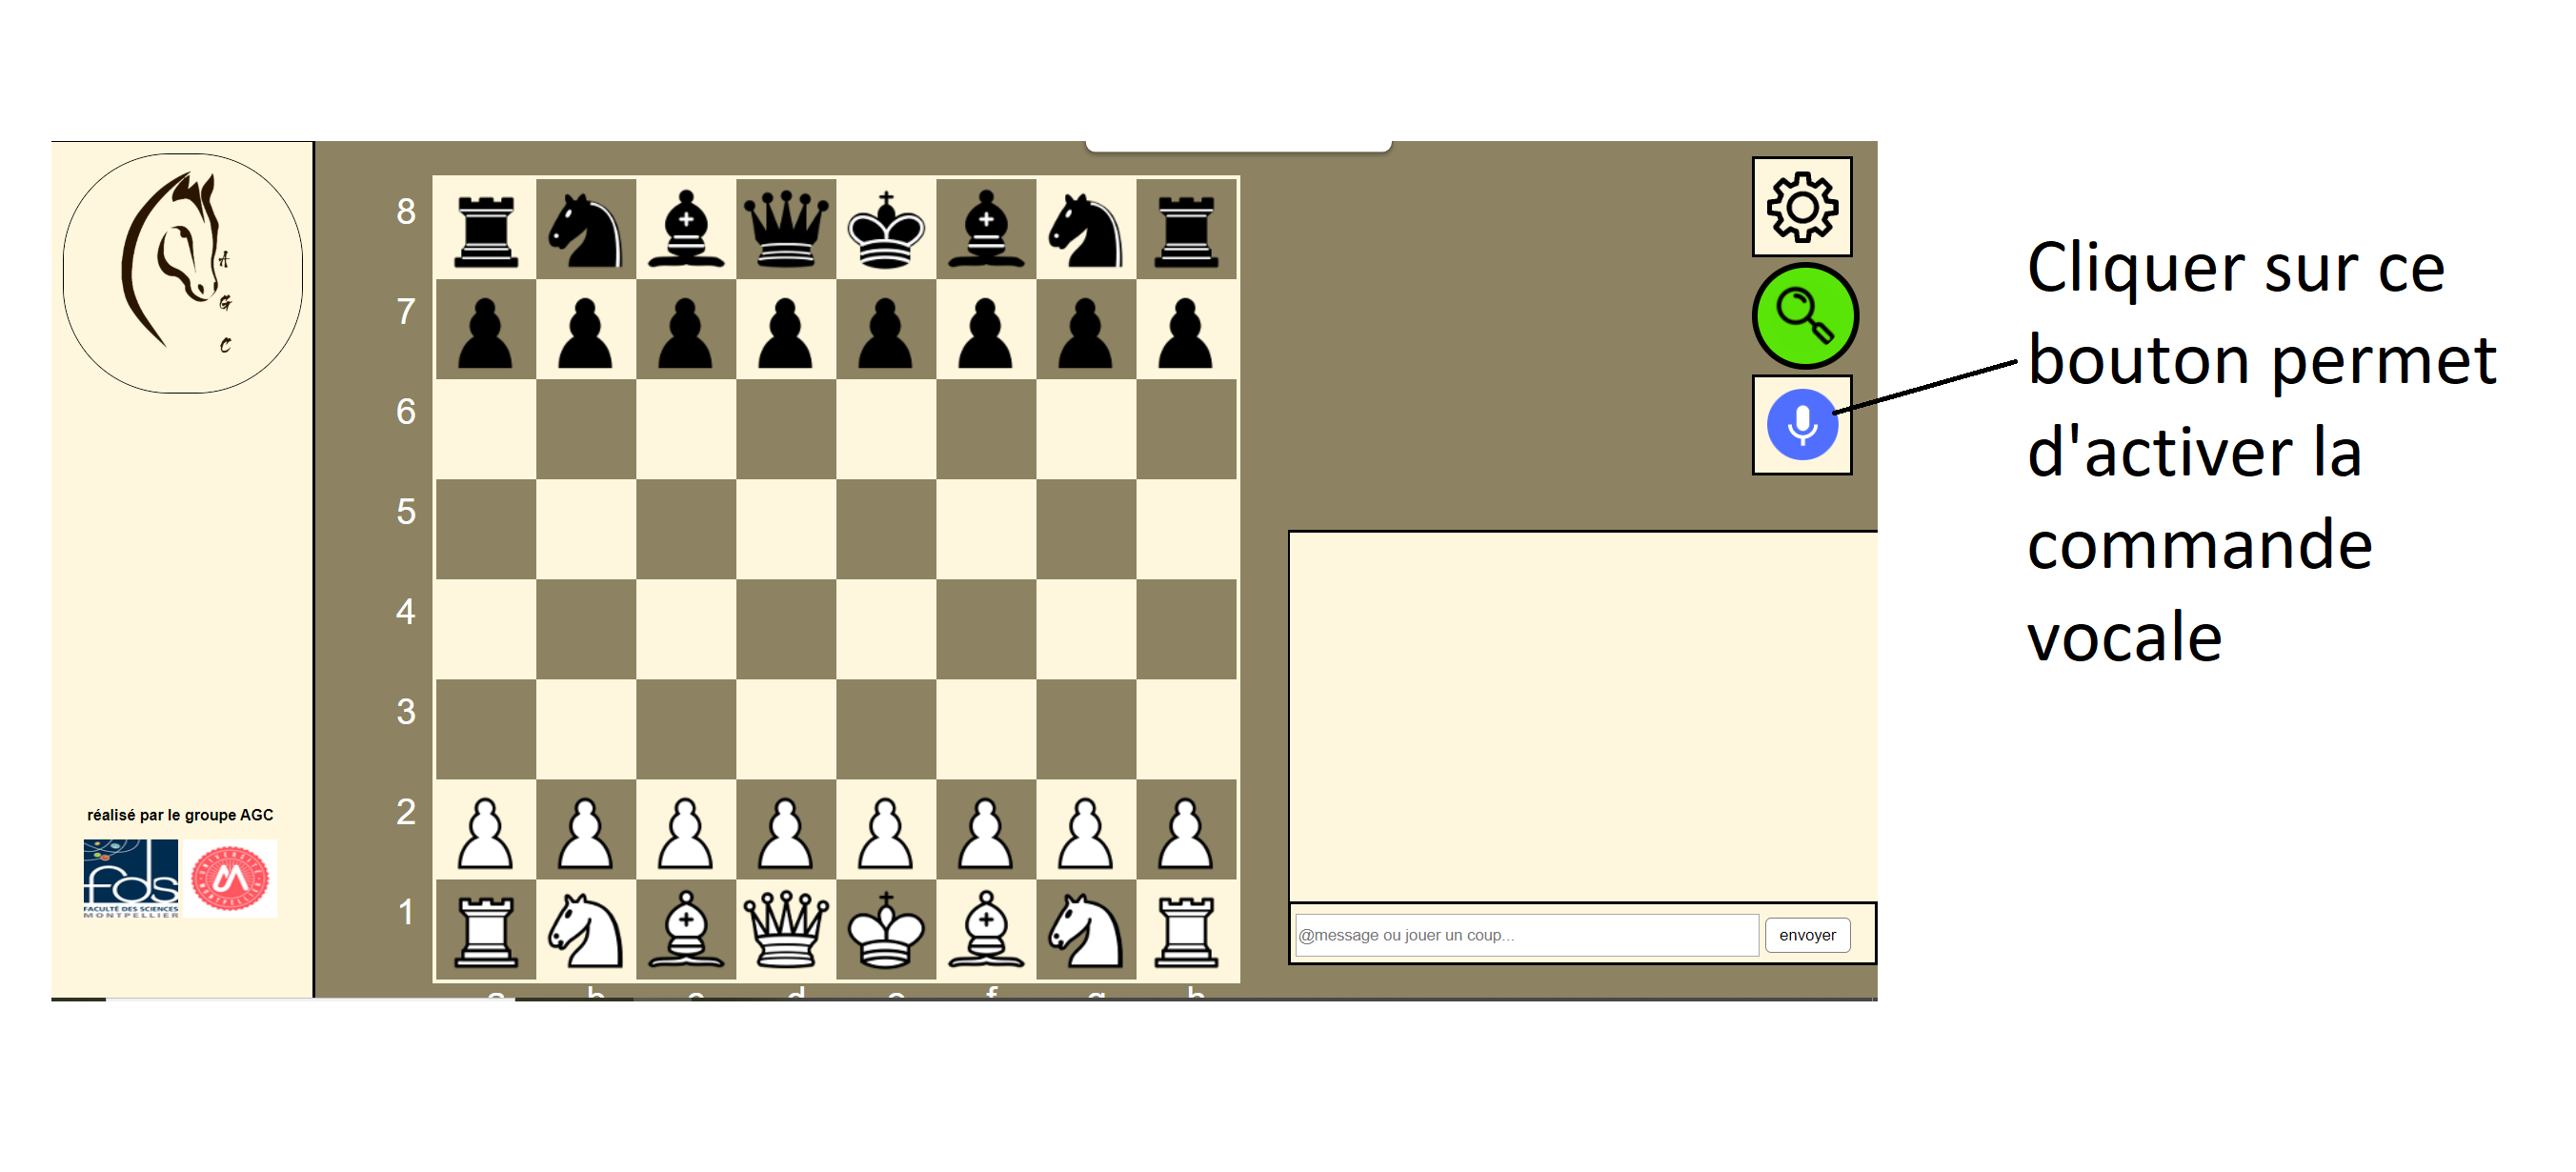
\includegraphics[width=11cm]{src/image9.png}

Ainsi, un aveugle ne peut pas jouer au jeu pour le moment, mais quelques modifications pourraient permettre de rendre ceci possible.


Les aveugles utilisent généralement une commande vocale continue sur leur ordinateur, il faudrait donc que celle-ci soit détectée par le programme afin de l'utiliser sans avoir besoin d'appuyer sur le bouton.
Sinon l'utilisation d'une touche du clavier pour déclencher la commande vocale serait également possible.

Il y aurait également d'autres choses à modifier comme l'interface pour lancer une partie. En effet, un aveugle ne serait pas capable de cliquer sur les différents boutons pour choisir sa couleur ou lancer la partie. Il faudrait donc par exemple utiliser une commande vocale pour ces fonctionnalités. Celle-ci pourrait se lancer lors de la connexion à la page ou via l'appui sur une touche du clavier.

\subsubsection{Assez Gros Chess comme plateforme de jeu d'échec pour malvoyant}

Nous pourrions modifier le programme afin de créer une plateforme de jeu d'échec en ligne pour les malvoyants à l'image de lichess.org (pour les joueurs voyants).

Nous avons essayé de mettre notre programme en ligne seulement, nous avons rencontré quelques problèmes.
\begin{itemize}
    \item Le programme actuel permet la création d'une seule partie de jeu, donc seuls deux joueurs peuvent jouer en même temps.
    \item La plupart des navigateurs comme chrome n'autorisent pas l'utilisation du microphone pour les sites non sécurisés, or notre site est actuellement en http donc non sécurisé.
\end{itemize}.

Afin de permettre la création de plusieurs sessions de jeu deux possibilités s'offrent à nous.

La première est de modifier le code du jeu en lui en même, en créant par exemple une classe session qui gère une session de jeu et on crée différentes instances de cette classe à la demande des utilisateurs.

La deuxième utilisée par de nombreux serveurs de jeu en ligne est de diviser les ressources entre différents serveurs de jeu qui sont reliés entre eux par un serveur proxy.

En ce qui concerne l'utilisation du microphone sur les navigateurs, il faut donc sécuriser le site en utilisant le protocole https. Pour cela, il faudra donc acquérir un certificat SSL chez un hébergeur .

\subsubsection{Utilisation d'Assez Gros Chess dans le développement d'autre jeux de plateau adaptés pour malvoyants}

En effet l'architecture actuelle d'Assez Gros Chess permettrait de développer d'autres jeux adaptés aux malvoyants comme le jeu de go, les dames...

Côté client, l'interface graphique demeurerait presque inchangée mise à part le plateau, les fonctionnalités de zoom, double confirmation, contrôle vocal, et même le chat peut être conservé.
Petit aperçu de Assez gros Checkers :

\begin{center}
\centering
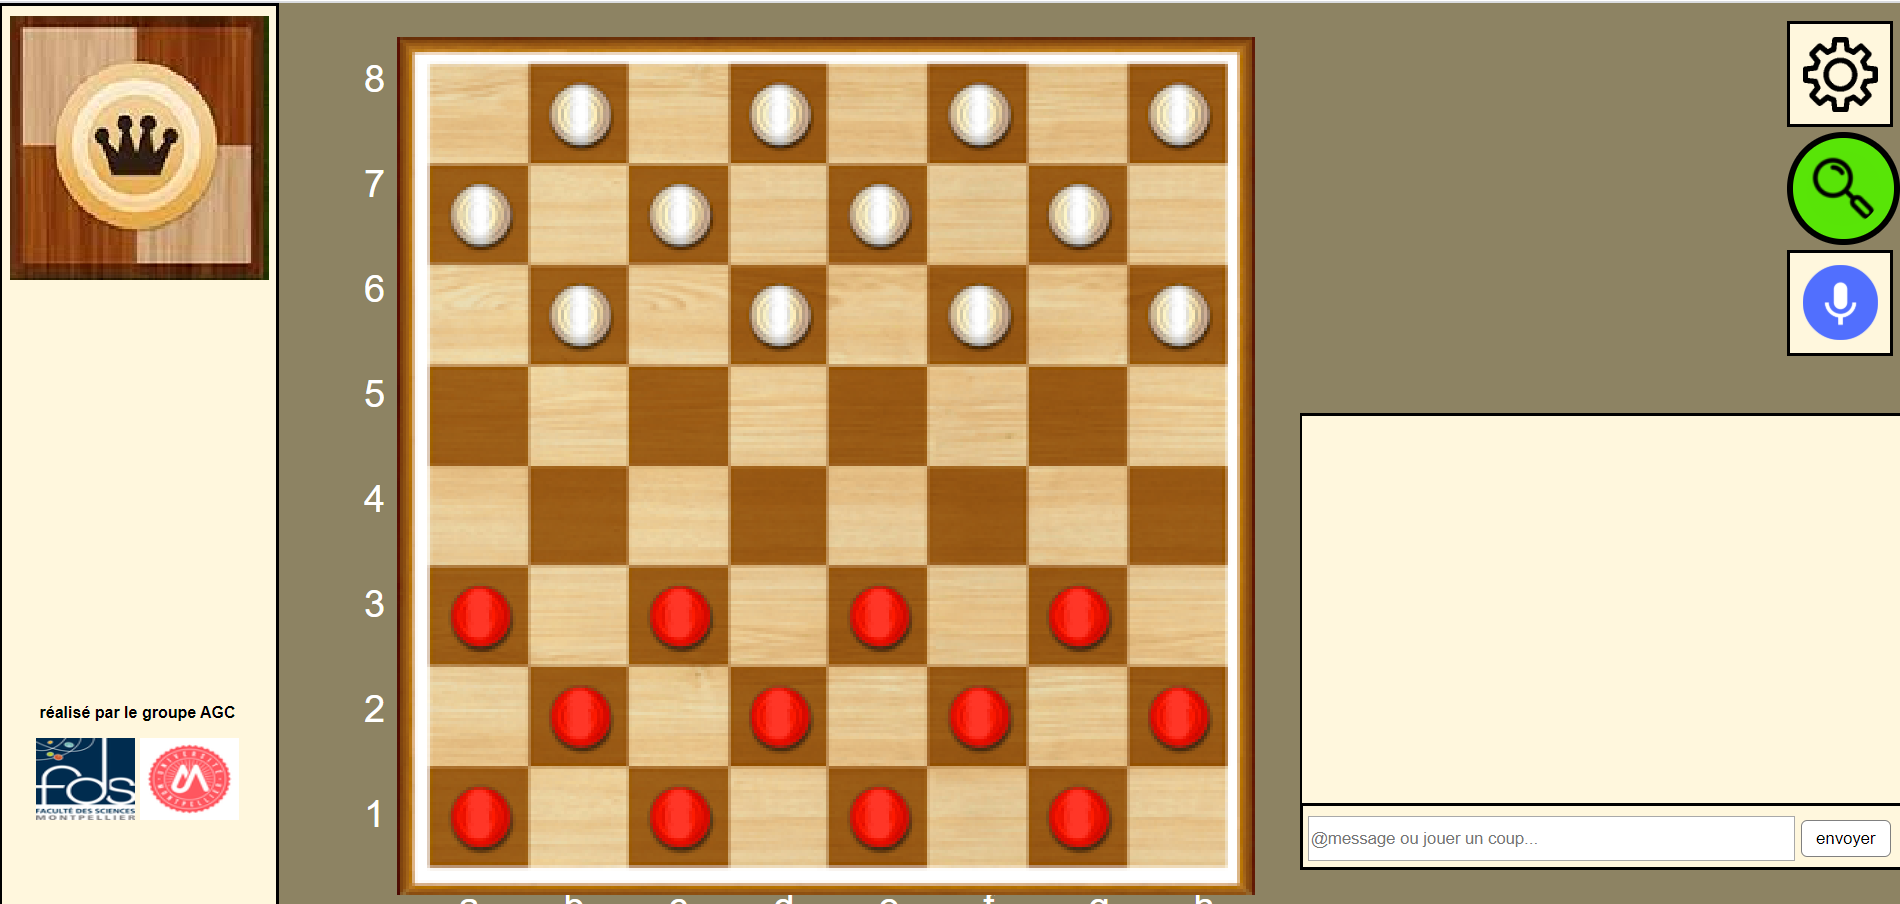
\includegraphics[width=14cm]{src/image10.png}    
\end{center}

Côté serveur les contrôleurs géreraient toujours le même type d'évènements : connexions, message du chat, nouveau coup...
Ils ont donc besoin de peu de modifications.
La plus grosse partie à modifier serait le modèle, puisqu'il s'agirait maintenant d'un jeu de dame ou de go et non plus d'un jeu d'échec, les règles seraient alors différentes.


\chapter{Conclusion}
Ce projet nous a permis de mettre en pratique et de consolider de nombreuses connaissances acquises tout au long de notre parcours universitaire. Nous donnons dans cette partie des exemples d’enseignements qui nous ont été utiles dans la réalisation de ce projet.\newline

Les cours de techniques de communication, de conduite de projets (HLIN408) nous ont permis d’appréhender la gestion du projet et d’apprendre à utiliser de nombreux outils utiles tels que LATEX et GitLab.

Grâce aux cours de modélisation et de programmation par objet (HLIN406) ainsi que ceux de programmation applicative avancée (HLIN302) nous avons appris la programmation orientée objet, ce qui nous permit de l’utiliser dans notre travail.

Nous avons également pu développer nos compétences en modélisation UML en utilisant nos cours de modélisation et de programmation par objet (HLIN406) ce qui nous a été très utile dans nos choix d ‘architecture pour notre site web.\newline 

Ce projet nous a également permis de développer de nouvelles compétences. En particulier la partie réseau qui était un domaine totalement inconnu pour nous. Nous avons également pu apprendre le Java Script, très utilisés dans le développement web.\newline

Grâce à ce projet chaque membre de l’équipe a pu renforcer ses connaissances mais aussi apporter son savoir et ses compétences aux autres membres afin d’harmoniser l’efficacité de l’équipe.
À travers des méthodes de travail et divers outils, ce projet nous a permis de nous immerger dans un univers professionnel.\newline

Il est vrai que de créer un site web et respecter un cahier des charges rendent un projet intéressant et professionnalisant, mais il y a aussi toutes les démarches qui ne sont pas visibles et qui rendent une telle expérience aussi enrichissante : écouter l’opinion de chacun des membres de l’équipe, savoir communiquer et argumenter afin d’opter pour les meilleurs choix, s’organiser sur les plans individuels et collectifs, gérer les imprévus, respecter des délais pour ne pas gêner ses collègues ni retarder le projet.\newline



\chapter{Annexes}

\textbf{3.2 - Schéma sur le fonctionnement des sockets}

\begin{center}
\centering
\fbox{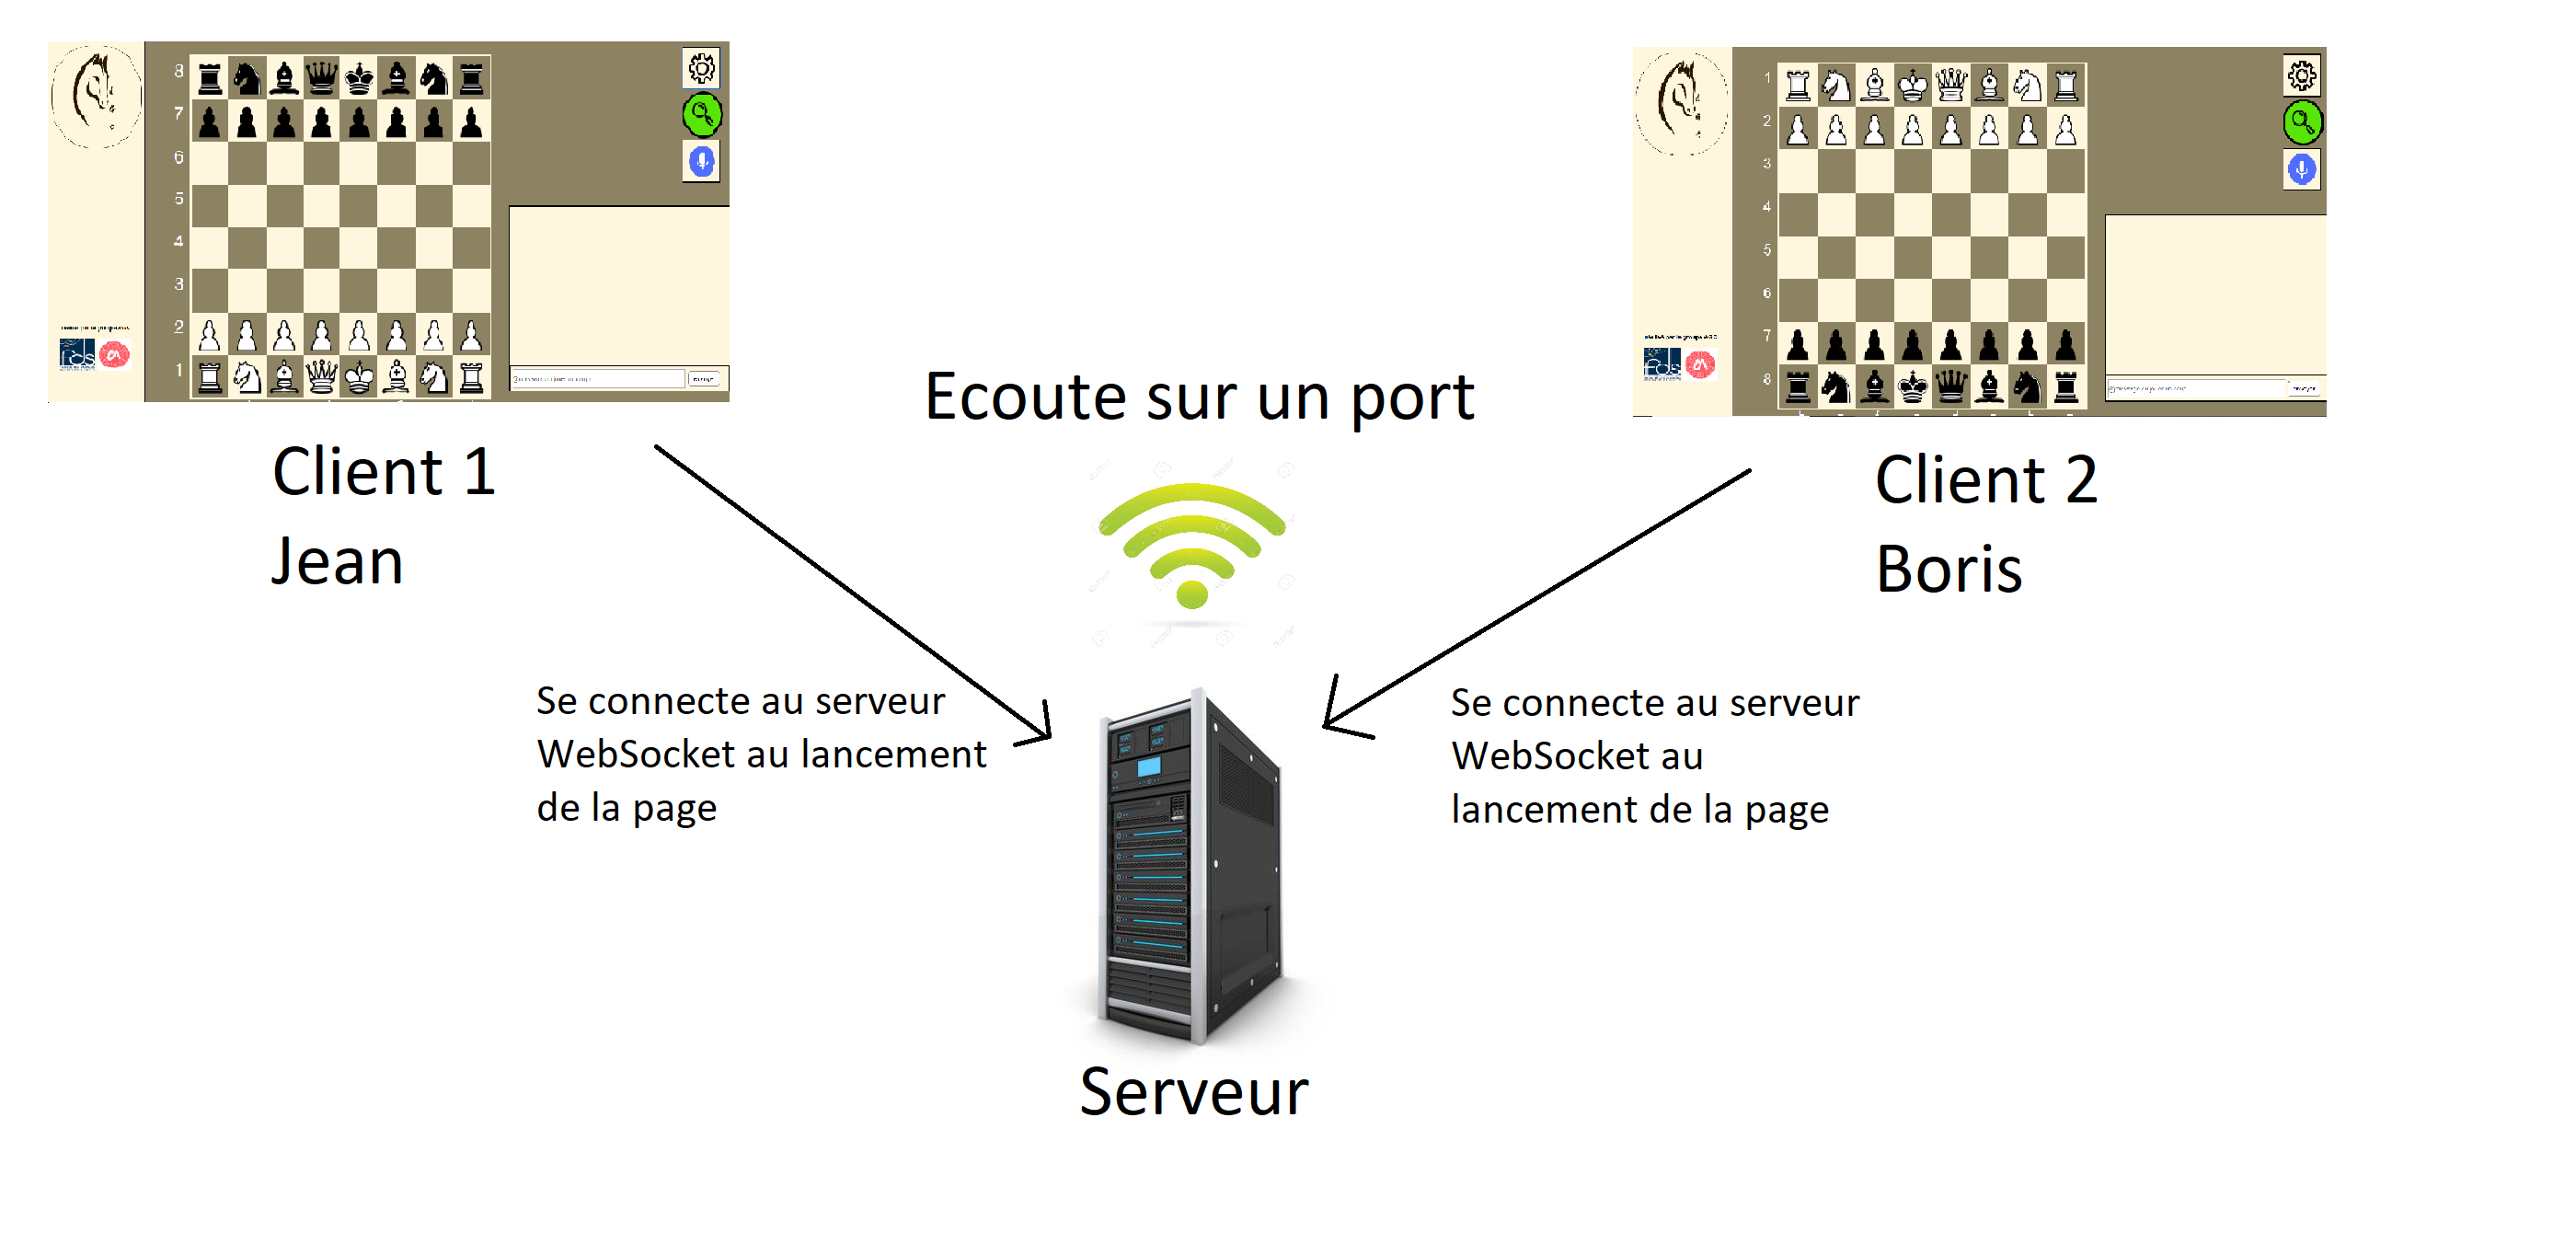
\includegraphics[width=16cm]{src/image1.png}}
\caption{Fig 1 . Connexions des clients au serveur Websocket}
\fbox{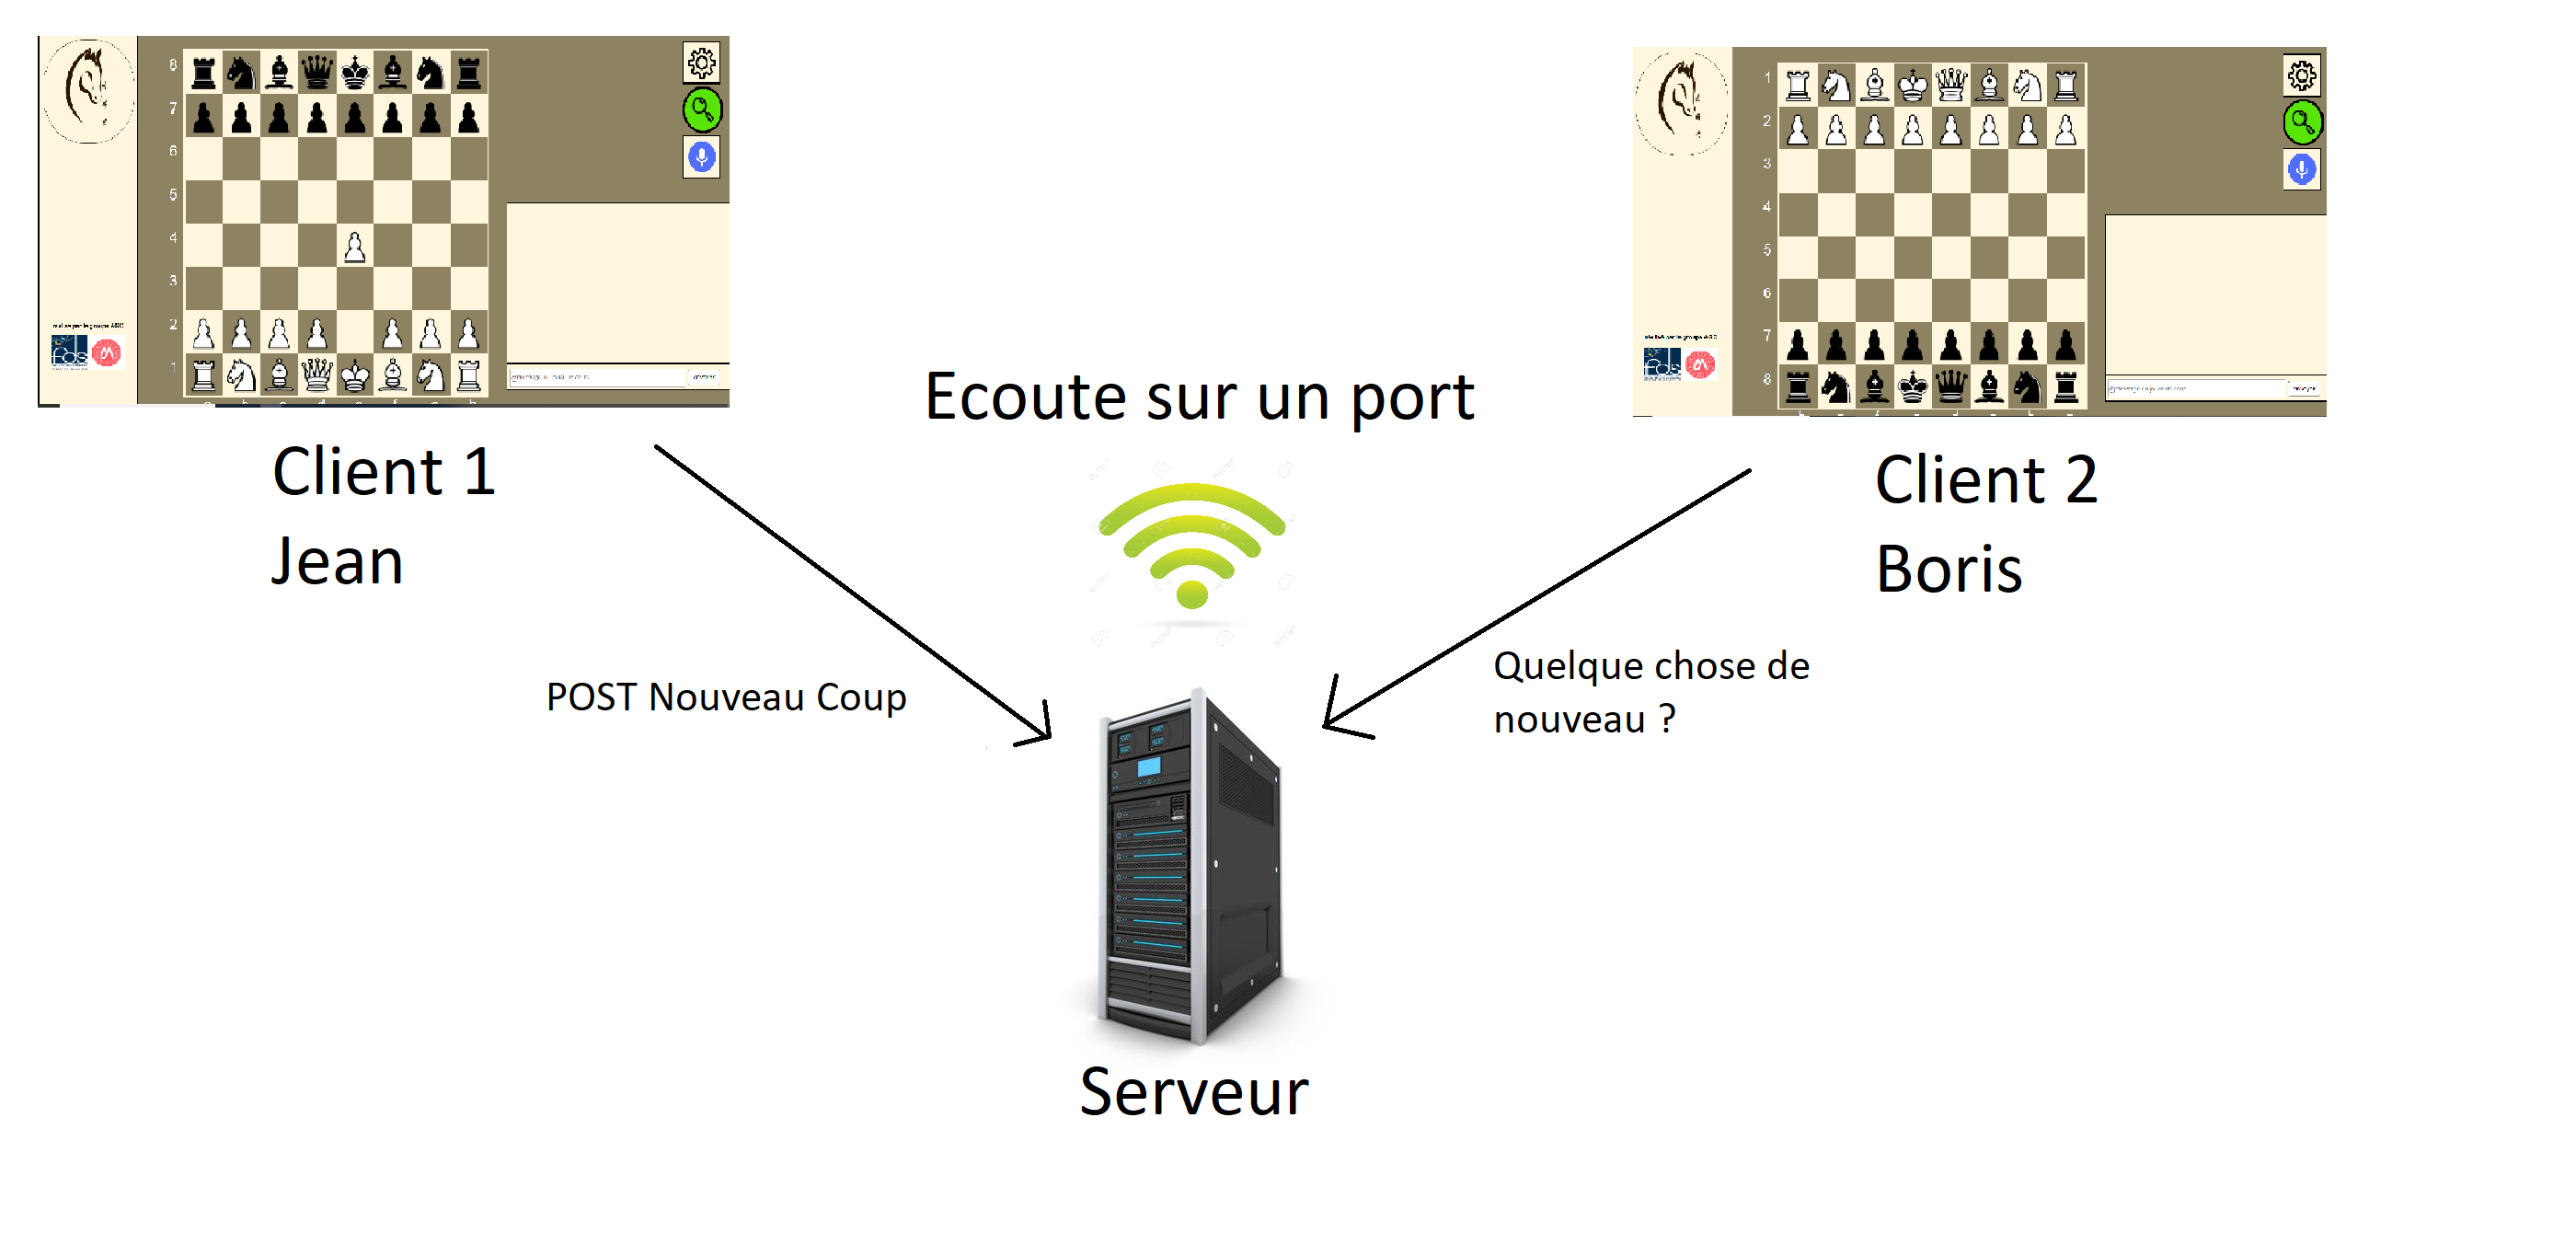
\includegraphics[width=16cm]{src/image2.png}}
\caption{Fig 2 . Le client 1 envoie une nouvelle information via la méthode POST, le client 2 est à
l’écoute de mise à jour}
\newline\newline
\fbox{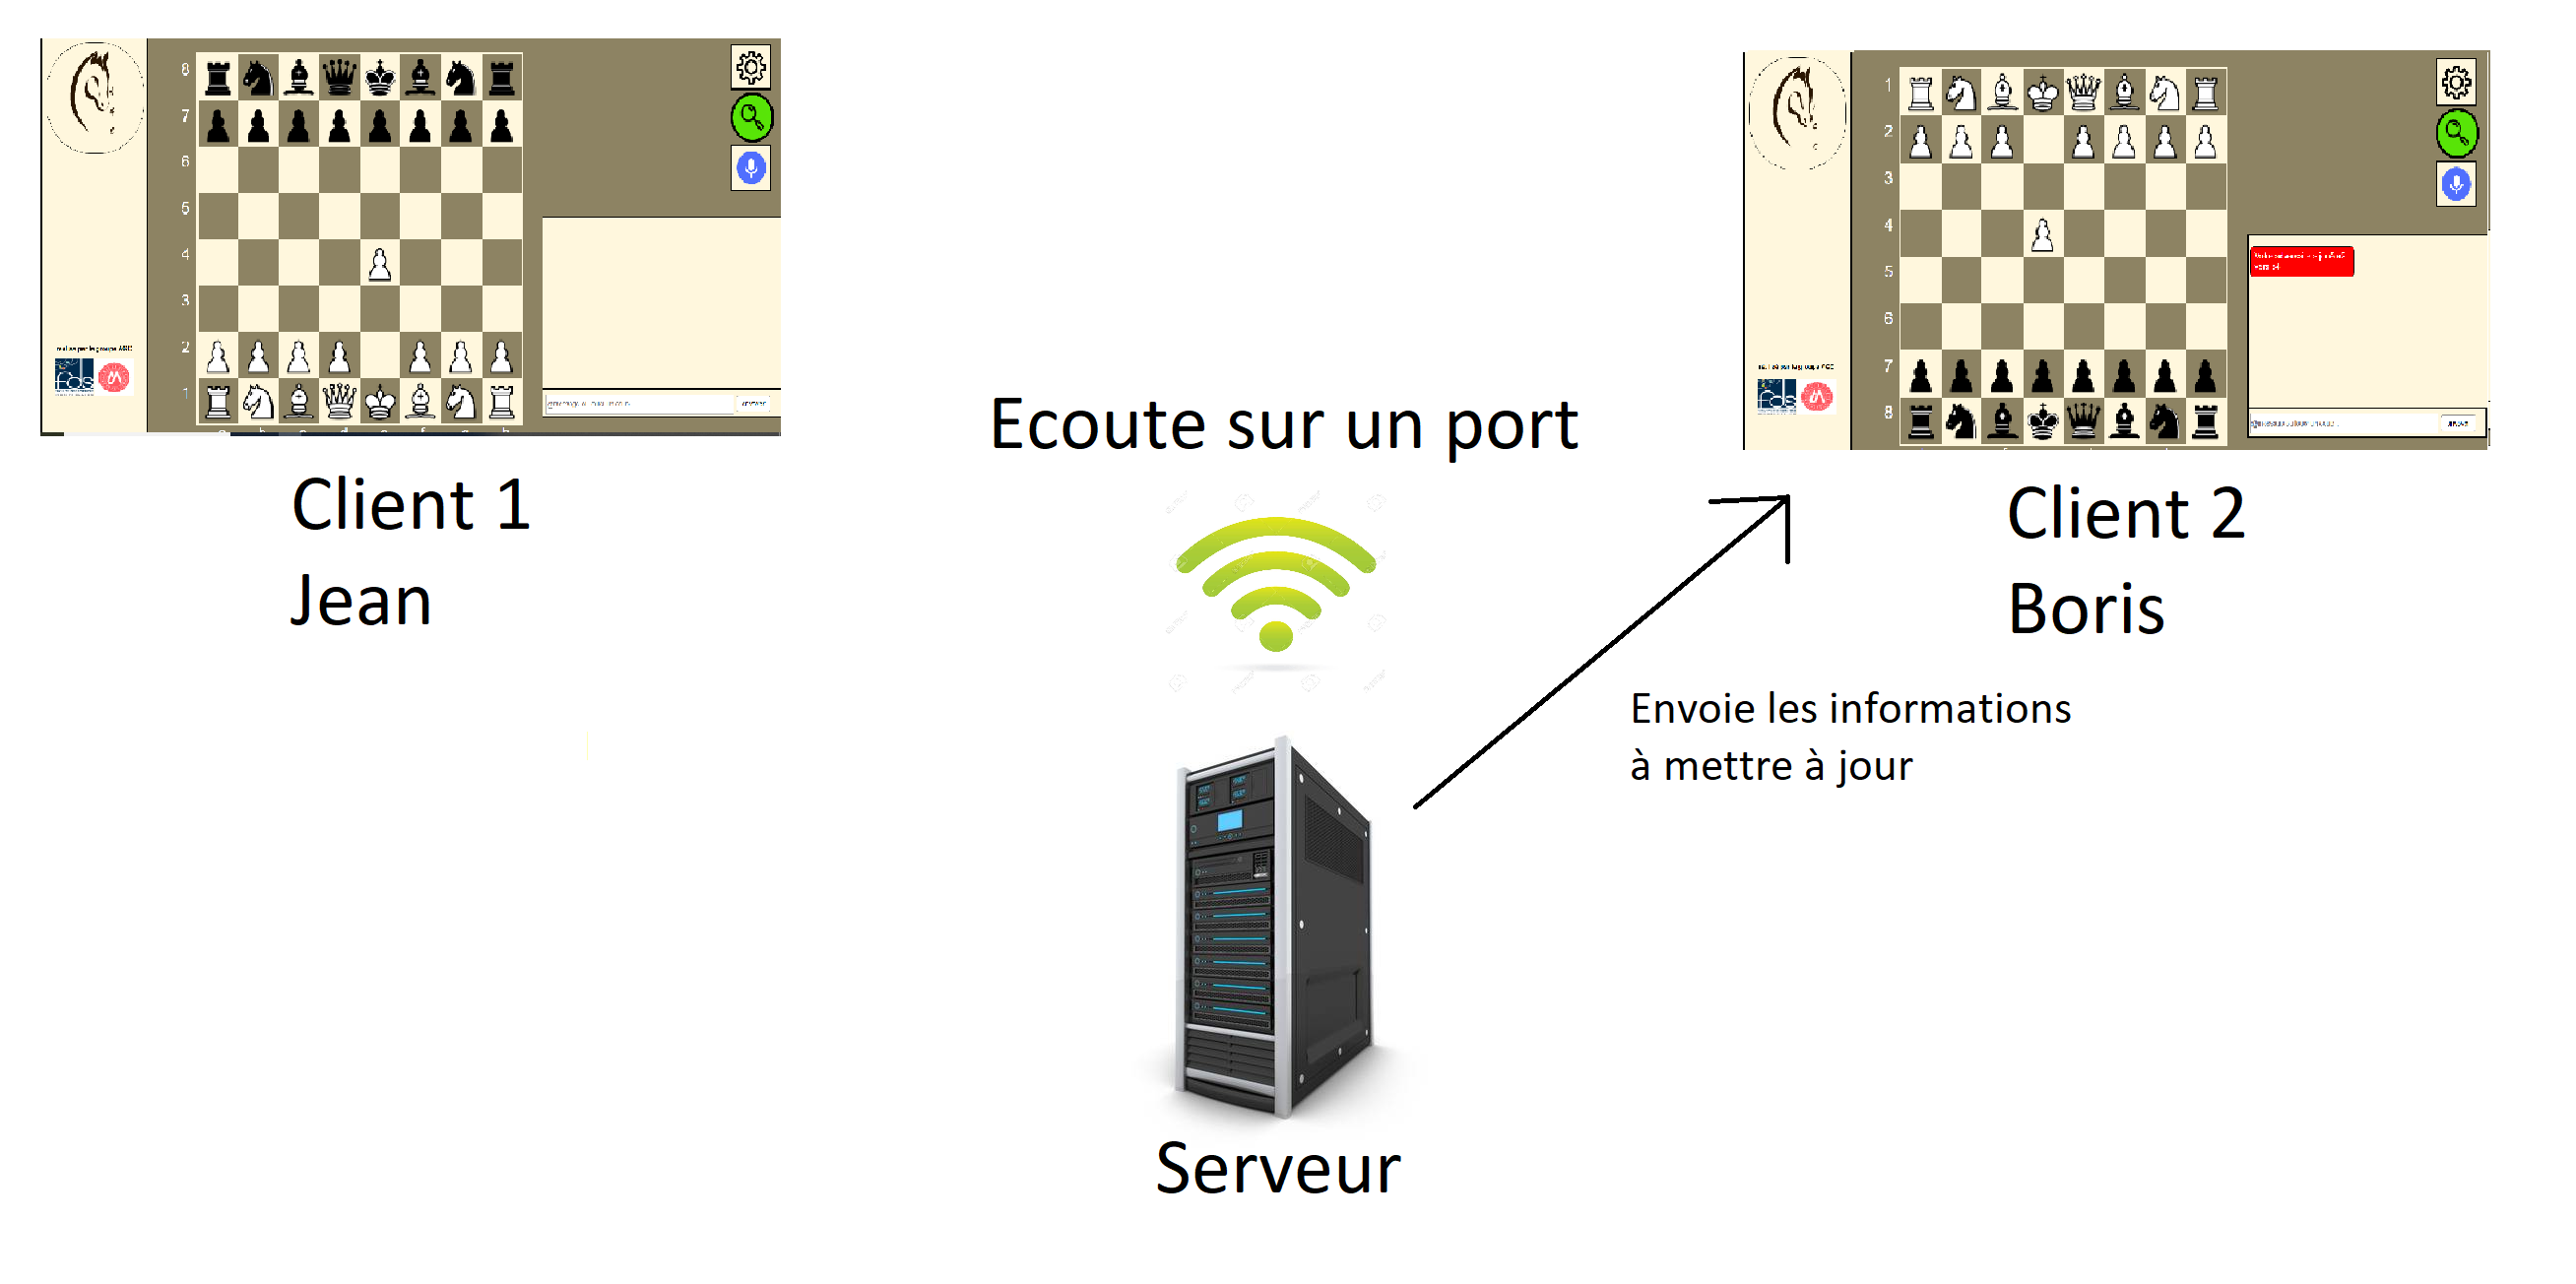
\includegraphics[width=16cm]{src/image3.png}}
\caption{Fig 3 . Les nouvelles informations sont envoyées au client 2}
\end{center}

\textbf{3.3.2 - Classe de gestion des évènements}

Le code ci-dessous est le code de la classe qui permet de réceptionner les évènements et de les "rediriger" vers leurs blocs respectifs.

\small
\begin{verbatim}
class GeneralController{

	constructor(){
		this.networkController = nC.networkController();
		this.chatController = cC.chatController();
		this.gameController = gaC.gameController();
	}

	handleEvent(socket){

		socket.on('couleur', (couleur) =>{
	        this.networkController.onChoixCouleur(couleur,socket);
	    });

	    socket.on('coGame', (pseudo) =>{
	        this.networkController.onCoGame(pseudo,socket);
	    });

	    socket.on('chat', (message) =>{
	        this.chatController.onMessage(socket,socket.player,message);
	    });

	    socket.on('listeCoups', (pos,couleur) =>{
	        this.gameController.onListeCoups(pos,socket,couleur);
	    });

	    socket.on('tourCourrant', () =>{
	        this.gameController.onTourCourrant(socket);
	    });

	    socket.on('coupPlateau', (coup) =>{
	        this.gameController.onCoupPlateau(coup,socket.player,socket);
	    });

	    socket.on('update', () =>{
	        this.gameController.onUpdate(socket);
	    });
	}

}
\end{verbatim}
\normalsize
\textbf{3.3.3 - Classe joueur}

Le code ci-dessous est le code de la classe joueur qui permet de retenir un certain nombre d'informations utiles concernant un joueur.

\footnotesize
\begin{verbatim}
class Player{

    constructor(idPlayer,couleur,pseudo){
       this.idPlayer = idPlayer;
	   this.couleur = couleur;
	   this.pseudo = pseudo;
    }

    status(){
	return this.pseudo + '(' + ((this.couleur == 'w') ? 'Blanc' : 'Noir') + ')';
    }

    setPseudo(pseudo){
    	this.pseudo = pseudo;
    }

    getPseudo(){
        return this.pseudo;
    }

    getCouleur(){
        return this.couleur;
    }
}
\end{verbatim}
\normalsize

\textbf{3.3.5 - Les fonctions d'analyse}

Les fonctions d'analyse vont permettre de filtrer le chat afin de retrouver des mots particuliers avec un sens important.

\footnotesize
\begin{verbatim}

includePieces(message){
	if(message.includes('pion')){
		return "";
	}else if(message.includes('tour')){
		return "R";
    }else if(message.includes('cavalier' ||  message.includes('chevalier'))){
    	return "N";
    }else if(message.includes('fou')){
    	return "B";
    }else if(message.includes('reine') || message.includes('dame')){
    	return "Q";
    }else if(message.includes('roi')){
    	return "K";
    }else{
		return null;
    }
}

includeSquare(message){

		let index = message.search(/[a-h][0-8]/);
		if(index!=-1)
			return message.substring(index, index+2);
		else
			return null;
	}
\end{verbatim}
\normalsize
\textbf{3.4.2 - Feuille de style du chat}

Le code ci-dessous écrit en css permet de gérer l'apparence du chat sur la page.

\begin{verbatim}
#chat_zone .console{
  background-color: red;
  border: solid black 1px;
  border-radius: 8px;
  padding: 8px;
  width: 40%;
  color: white;
}
#chat_zone .recu{
  background-color: white;
  border: solid black 1px;
  border-radius: 8px;
  padding: 8px;
  width: 40%;
}
#chat_zone .emis{
  background-color: skyblue;
  border: solid black 1px;
  border-radius: 8px;
  padding: 8px;
  width: 40%;
  margin-left: 50%;
}
\end{verbatim}
\textbf{3.4.3 - Reconnaissance Vocale}

Ce code permet de transformer une instruction vocale en chaîne de texte.

\begin{verbatim}
var recognition = new webkitSpeechRecognition();
recognition.lang = 'fr';
recognition.interimResults = false;
recognition.maxAlternatives = 1;

function reconnaissanceVocale(){
    recognition.start();
    console.log('listening....');
}

recognition.onresult = function(event) {
    let msg = event.results[0][0].transcript;
    $('#chat_zone').append('<p class="emis">'+msg+'</p>');
    socket.emit('chat', msg);
}
\end{verbatim}
\textbf{Synthèse Vocale}

Ce code permet de lire une chaîne de texte.

\begin{verbatim}
if(message.sender!=col && lectureMessage){// est vocale activé 
    let speech = new SpeechSynthesisUtterance(message.vocale);
    speech.lang = "fr";
    window.speechSynthesis.speak(speech);
  }
\end{verbatim}
\textbf{3.4.4 - Fonctions de grossissement}

Les fonctions JavaScript ci-dessous permettent le zoom sur les différents éléments de la page lorsqu'on les survole.

\begin{verbatim}
         $('#Update2').mouseover(function(){
         	if(zoomB){
	         	$(this).css('transform', 'scale(1.3 , 1.3)');
    	     	$(this).css('transform-origin', 'bottom right');
    	     }
         });

         $('#Update2').mouseout(function(){
         	$(this).css('transform', 'scale(1 , 1)');
         });

         $('#maskey').mouseover(function(){
         	if(zoomB){
	         	$(this).css('transform', 'scale(1.3 , 1.3)');
    	     	$(this).css('transform-origin', 'top right');
    	     }
         });

         $('#maskey').mouseout(function(){
         	$(this).css('transform', 'scale(1 , 1)');
         });

         $('.para').mouseover(function(){
         	if(zoomB){
	         	$(this).css('transform', 'scale(1.2 , 1.2)');
    	     }
         });

         $('.para').mouseout(function(){
         	$(this).css('transform', 'scale(1 , 1)');
         });
\end{verbatim}

\chapter{Quelques sources}

\begin{itemize}
    \item Général \begin{itemize}
        \item Prise en main de NodeJS
https://openclassrooms.com/fr/courses/1056721-des-applications-ultra-rapides-avec-node-js
        \item Documentation javascript : w3schools.com/js
    \end{itemize}
    \item Paramètres \begin{itemize}
        \item Zoom Police :
https://forum.alsacreations.com/topic-5-83433-1-Fonction-zoom.html
    \item Zoom :
http://burnignorance.com/javascript-performance-tips/zooming-a-web-page-using-javascript-functions/
    \end{itemize}
    \item API \begin{itemize}
        \item Chess.js :
https://www.npmjs.com/package/chess.js
        \item Commande Vocale :
https://developer.mozilla.org/fr/docs/Web/API/Web\_Speech\_API
    \end{itemize}
    \item Déficiences Visuelles \begin{itemize}
        \item Daltonisme :
https://www.zeiss.fr/vision-care/mieux-voir/comprendre-la-vision/deficience-rouge-vert-daltonisme-rouge-vert-et-daltonisme-total.html
    \end{itemize}
\end{itemize}

\end{document}
